%%%%%%%%%%%%%%%%%%%%%%%%%%%%%%%%%%%%%%%%%%%%%%%%%%%%%%%%%%%%%%%%%%%%%%%%%%%%%%%%%%%%%%%%%%%%%%%%%%%%%%%%%%%%%%%%%%%%%%%%%%%%%%%%%%%%%%%%%%%%%%%%%%%%%%%%%%%
%DIF LATEXDIFF DIFFERENCE FILE
%DIF DEL Manu_article_V1.tex   Wed Jul 28 23:23:48 2021
%DIF ADD Manu_article_V2.tex   Wed Aug  4 22:19:09 2021
% This is just an example/guide for you to refer to when submitting manuscripts to Frontiers, it is not mandatory to use Frontiers .cls files nor frontiers.tex  %
% This will only generate the Manuscript, the final article will be typeset by Frontiers after acceptance.
%                                              %
%                                                                                                                                                         %
% When submitting your files, remember to upload this *tex file, the pdf generated with it, the *bib file (if bibliography is not within the *tex) and all the figures.
%%%%%%%%%%%%%%%%%%%%%%%%%%%%%%%%%%%%%%%%%%%%%%%%%%%%%%%%%%%%%%%%%%%%%%%%%%%%%%%%%%%%%%%%%%%%%%%%%%%%%%%%%%%%%%%%%%%%%%%%%%%%%%%%%%%%%%%%%%%%%%%%%%%%%%%%%%%

%%% Version 3.4 Generated 2018/06/15 %%%
%%% You will need to have the following packages installed: datetime, fmtcount, etoolbox, fcprefix, which are normally inlcuded in WinEdt. %%%
%%% In http://www.ctan.org/ you can find the packages and how to install them, if necessary. %%%

\documentclass[utf8]{frontiersSCNS}

%\setcitestyle{square} % for Physics and Applied Mathematics and Statistics articles
\usepackage{url,hyperref,lineno,microtype,subcaption}
\usepackage[onehalfspacing]{setspace}

\linenumbers


% BELOW TAKEN FROM rticles plos template
%
% amsmath package, useful for mathematical formulas
\usepackage{amsmath}
% amssymb package, useful for mathematical symbols
\usepackage{amssymb}

% hyperref package, useful for hyperlinks
\usepackage{hyperref}

% graphicx package, useful for including eps and pdf graphics
% include graphics with the command \includegraphics
\usepackage{graphicx}

% Sweave(-like)
\usepackage{fancyvrb}
\DefineVerbatimEnvironment{Sinput}{Verbatim}{fontshape=sl}
\DefineVerbatimEnvironment{Soutput}{Verbatim}{}
\DefineVerbatimEnvironment{Scode}{Verbatim}{fontshape=sl}
\newenvironment{Schunk}{}{}
\DefineVerbatimEnvironment{Code}{Verbatim}{}
\DefineVerbatimEnvironment{CodeInput}{Verbatim}{fontshape=sl}
\DefineVerbatimEnvironment{CodeOutput}{Verbatim}{}
\newenvironment{CodeChunk}{}{}

% cite package, to clean up citations in the main text. Do not remove.
\usepackage{cite}

\usepackage{color}

\providecommand{\tightlist}{%
  \setlength{\itemsep}{0pt}\setlength{\parskip}{0pt}}

% Below is from frontiers
%
\bibliographystyle{frontiersinSCNS}
% Use doublespacing - comment out for single spacing
%\usepackage{setspace}
%\doublespacing


% Leave a blank line between paragraphs instead of using \\


\def\keyFont{\fontsize{8}{11}\helveticabold }


%% ** EDIT HERE **
%% PLEASE INCLUDE ALL MACROS BELOW

%% END MACROS SECTION

% Pandoc citation processing
\newlength{\csllabelwidth}
\setlength{\csllabelwidth}{3em}
\newlength{\cslhangindent}
\setlength{\cslhangindent}{1.5em}
% for Pandoc 2.8 to 2.10.1
\newenvironment{cslreferences}%
  {}%
  {\par}
% For Pandoc 2.11+
\newenvironment{CSLReferences}[2] % #1 hanging-ident, #2 entry spacing
 {% don't indent paragraphs
  \setlength{\parindent}{0pt}
  % turn on hanging indent if param 1 is 1
  \ifodd #1 \everypar{\setlength{\hangindent}{\cslhangindent}}\ignorespaces\fi
  % set entry spacing
  \ifnum #2 > 0
  \setlength{\parskip}{#2\baselineskip}
  \fi
 }%
 {}
\usepackage{calc} % for calculating minipage widths
\newcommand{\CSLBlock}[1]{#1\hfill\break}
\newcommand{\CSLLeftMargin}[1]{\parbox[t]{\csllabelwidth}{#1}}
\newcommand{\CSLRightInline}[1]{\parbox[t]{\linewidth - \csllabelwidth}{#1}\break}
\newcommand{\CSLIndent}[1]{\hspace{\cslhangindent}#1}
\usepackage{pdflscape}
\newcommand{\blandscape}{\begin{landscape}}
\newcommand{\elandscape}{\end{landscape}}


\def\Authors{
  Chaochen Wang\,\textsuperscript{1},
  Suzana Almoosawi\,\textsuperscript{2},
  Luigi Palla\,\textsuperscript{3,4,5*}}

\def\Address{

  \textsuperscript{1} Department of Public Health, Aichi Medical
University,  Nagakute,  Aichi,  Japan
  
  \textsuperscript{2} Faculty of Medicine, School of Public
Health, Imperial College London,  London,   UK
  
  \textsuperscript{3} Department of Public Health and Infectious
Diseases, University of Rome La Sapienza,  Rome,   Italy
  
  \textsuperscript{4} Department of Medical Statistics, London School of
Hygiene \& Tropical Medicine,  London,   UK
  
  \textsuperscript{5} Department of Global Health, School of Tropical
Medicine and Global Health, University of Nagasaki,  Nagasaki,   Japan
  }

  
  \def\firstAuthorLast{WANG {et~al.}}
  
  
  \def\corrAuthor{Luigi Palla}\def\corrAddress{Department of Public
Health and Infectious Diseases, University of Rome La Sapienza\\Piazzale
Aldo Moro
5\\Rome, 00185 Italy}\def\corrEmail{\href{mailto:Luigi.Palla@uniroma1.it}{\nolinkurl{Luigi.Palla@uniroma1.it}}}
  
%DIF PREAMBLE EXTENSION ADDED BY LATEXDIFF
%DIF UNDERLINE PREAMBLE %DIF PREAMBLE
\RequirePackage[normalem]{ulem} %DIF PREAMBLE
\RequirePackage{color}\definecolor{RED}{rgb}{1,0,0}\definecolor{BLUE}{rgb}{0,0,1} %DIF PREAMBLE
\providecommand{\DIFaddtex}[1]{{\protect\color{blue}\uwave{#1}}} %DIF PREAMBLE
\providecommand{\DIFdeltex}[1]{{\protect\color{red}\sout{#1}}}                      %DIF PREAMBLE
%DIF SAFE PREAMBLE %DIF PREAMBLE
\providecommand{\DIFaddbegin}{} %DIF PREAMBLE
\providecommand{\DIFaddend}{} %DIF PREAMBLE
\providecommand{\DIFdelbegin}{} %DIF PREAMBLE
\providecommand{\DIFdelend}{} %DIF PREAMBLE
\providecommand{\DIFmodbegin}{} %DIF PREAMBLE
\providecommand{\DIFmodend}{} %DIF PREAMBLE
%DIF FLOATSAFE PREAMBLE %DIF PREAMBLE
\providecommand{\DIFaddFL}[1]{\DIFadd{#1}} %DIF PREAMBLE
\providecommand{\DIFdelFL}[1]{\DIFdel{#1}} %DIF PREAMBLE
\providecommand{\DIFaddbeginFL}{} %DIF PREAMBLE
\providecommand{\DIFaddendFL}{} %DIF PREAMBLE
\providecommand{\DIFdelbeginFL}{} %DIF PREAMBLE
\providecommand{\DIFdelendFL}{} %DIF PREAMBLE
%DIF HYPERREF PREAMBLE %DIF PREAMBLE
\providecommand{\DIFadd}[1]{\texorpdfstring{\DIFaddtex{#1}}{#1}} %DIF PREAMBLE
\providecommand{\DIFdel}[1]{\texorpdfstring{\DIFdeltex{#1}}{}} %DIF PREAMBLE
\newcommand{\DIFscaledelfig}{0.5}
%DIF HIGHLIGHTGRAPHICS PREAMBLE %DIF PREAMBLE
\RequirePackage{settobox} %DIF PREAMBLE
\RequirePackage{letltxmacro} %DIF PREAMBLE
\newsavebox{\DIFdelgraphicsbox} %DIF PREAMBLE
\newlength{\DIFdelgraphicswidth} %DIF PREAMBLE
\newlength{\DIFdelgraphicsheight} %DIF PREAMBLE
% store original definition of \includegraphics %DIF PREAMBLE
\LetLtxMacro{\DIFOincludegraphics}{\includegraphics} %DIF PREAMBLE
\newcommand{\DIFaddincludegraphics}[2][]{{\color{blue}\fbox{\DIFOincludegraphics[#1]{#2}}}} %DIF PREAMBLE
\newcommand{\DIFdelincludegraphics}[2][]{% %DIF PREAMBLE
\sbox{\DIFdelgraphicsbox}{\DIFOincludegraphics[#1]{#2}}% %DIF PREAMBLE
\settoboxwidth{\DIFdelgraphicswidth}{\DIFdelgraphicsbox} %DIF PREAMBLE
\settoboxtotalheight{\DIFdelgraphicsheight}{\DIFdelgraphicsbox} %DIF PREAMBLE
\scalebox{\DIFscaledelfig}{% %DIF PREAMBLE
\parbox[b]{\DIFdelgraphicswidth}{\usebox{\DIFdelgraphicsbox}\\[-\baselineskip] \rule{\DIFdelgraphicswidth}{0em}}\llap{\resizebox{\DIFdelgraphicswidth}{\DIFdelgraphicsheight}{% %DIF PREAMBLE
\setlength{\unitlength}{\DIFdelgraphicswidth}% %DIF PREAMBLE
\begin{picture}(1,1)% %DIF PREAMBLE
\thicklines\linethickness{2pt} %DIF PREAMBLE
{\color[rgb]{1,0,0}\put(0,0){\framebox(1,1){}}}% %DIF PREAMBLE
{\color[rgb]{1,0,0}\put(0,0){\line( 1,1){1}}}% %DIF PREAMBLE
{\color[rgb]{1,0,0}\put(0,1){\line(1,-1){1}}}% %DIF PREAMBLE
\end{picture}% %DIF PREAMBLE
}\hspace*{3pt}}} %DIF PREAMBLE
} %DIF PREAMBLE
\LetLtxMacro{\DIFOaddbegin}{\DIFaddbegin} %DIF PREAMBLE
\LetLtxMacro{\DIFOaddend}{\DIFaddend} %DIF PREAMBLE
\LetLtxMacro{\DIFOdelbegin}{\DIFdelbegin} %DIF PREAMBLE
\LetLtxMacro{\DIFOdelend}{\DIFdelend} %DIF PREAMBLE
\DeclareRobustCommand{\DIFaddbegin}{\DIFOaddbegin \let\includegraphics\DIFaddincludegraphics} %DIF PREAMBLE
\DeclareRobustCommand{\DIFaddend}{\DIFOaddend \let\includegraphics\DIFOincludegraphics} %DIF PREAMBLE
\DeclareRobustCommand{\DIFdelbegin}{\DIFOdelbegin \let\includegraphics\DIFdelincludegraphics} %DIF PREAMBLE
\DeclareRobustCommand{\DIFdelend}{\DIFOaddend \let\includegraphics\DIFOincludegraphics} %DIF PREAMBLE
\LetLtxMacro{\DIFOaddbeginFL}{\DIFaddbeginFL} %DIF PREAMBLE
\LetLtxMacro{\DIFOaddendFL}{\DIFaddendFL} %DIF PREAMBLE
\LetLtxMacro{\DIFOdelbeginFL}{\DIFdelbeginFL} %DIF PREAMBLE
\LetLtxMacro{\DIFOdelendFL}{\DIFdelendFL} %DIF PREAMBLE
\DeclareRobustCommand{\DIFaddbeginFL}{\DIFOaddbeginFL \let\includegraphics\DIFaddincludegraphics} %DIF PREAMBLE
\DeclareRobustCommand{\DIFaddendFL}{\DIFOaddendFL \let\includegraphics\DIFOincludegraphics} %DIF PREAMBLE
\DeclareRobustCommand{\DIFdelbeginFL}{\DIFOdelbeginFL \let\includegraphics\DIFdelincludegraphics} %DIF PREAMBLE
\DeclareRobustCommand{\DIFdelendFL}{\DIFOaddendFL \let\includegraphics\DIFOincludegraphics} %DIF PREAMBLE
%DIF END PREAMBLE EXTENSION ADDED BY LATEXDIFF

\begin{document}
\onecolumn
\firstpage{1}

\title[Food groups choice and time of consumption.]{Relationships
between food groups and eating time slots according to diabetes status
in adults from the UK National Diet and Nutrition Survey (2008--2017)}
\author[\firstAuthorLast]{\Authors}
\address{} %This field will be automatically populated
\correspondance{} %This field will be automatically populated

\extraAuth{}% If there are more than 1 corresponding author, comment this line and uncomment the next one.
%\extraAuth{corresponding Author2 \\ Laboratory X2, Institute X2, Department X2, Organization X2, Street X2, City X2 , State XX2 (only USA, Canada and Australia), Zip Code2, X2 Country X2, email2@uni2.edu}


\maketitle

\begin{abstract}

Time of eating has been shown to be associated with diabetes and obesity but little is known about less healthy foods and specific time of their intake over the 24 hours of the day. In this study we aimed to identify potential relationships between foods and their eating time, and see whether these associations may vary by diabetes status. The National Diet and Nutrition Survey (NDNS) including 6802 adults (age $\geq$ 19 years old) collected 749,026 food recordings by a 4-day-diary. The contingency table cross-classifying 60 food groups with 7 pre-defined eating time slots (6-9am, 9am-12pm, 12-2pm, 2-5pm, 8-10pm, 10pm-6am) was analyzed by Correspondence Analysis (CA). CA biplots displaying the associations were generated for all adults and separately by diabetes status (self-reported, pre-diabetes, undiagnosed-diabetes, and non-diabetics) to visually explore the associations between food groups and time of eating across diabetes strata. For selected food groups, odds ratios (OR, 99\% confidence intervals, CI) were derived of consuming unhealthy foods at evening/night (8pm-6am) vs. earlier time in the day, by logistic regression models with generalized estimating equations. The biplots suggested positive associations between evening/night and consumption of puddings, regular soft drinks, sugar confectioneries, chocolates,  beers, ice cream, biscuits, and crisps for all adults in the UK. The OR (99\% CIs) of consuming these foods at evening/night were respectively 1.43 (1.06, 1.94), 1.72 (1.44, 2.05), 1.84 (1.31, 2.59), 3.08 (2.62, 3.62), 7.26 (5.91, 8.92), 2.45 (1.84, 3.25), 1.90 (1.68, 2.16), 1.49 (1.22, 1.82) vs. earlier time in the day adjusted for age, sex, body mass index, and social-economic levels. Stratified biplots found that sweetened beverages, sugar-confectioneries appeared more strongly associated with evening/night among un-diagnosed diabetics. Foods consumed in the evening/night time tend to be highly processed, easily accessible, and rich in added sugar or saturated fat. Individuals with undiagnosed diabetes are more likely to consume unhealthy foods at night. Further longitudinal studies are required to ascertain the causal direction of the association between late-eating and diabetes status.
\tiny
 \keyFont{ \section{Keywords:} Chrononutrition, time of eating, correspondence analysis, the UK National Diet and Nutrition Survey, nutrition epidemiology, diabetes} 

\end{abstract}

\hypertarget{introduction}{%
\section*{Introduction}\label{introduction}}
\addcontentsline{toc}{section}{Introduction}

The timing of energy intake has been shown to be associated with obesity
and diabetes. (Almoosawi et al., 2016) Specifically, eating late at
night or having a late dinner was found to be related to higher risk of
obesity (Xiao et al., 2019; Yoshida et al., 2018), hyperglycemia
(Nakajima and Suwa, 2015), metabolic syndrome (Kutsuma et al., 2014),
diabetes (Mattson et al., 2014), and poorer glycemic control among
diabetics (Sakai et al., 2017). However, the relationship between food
choice and the time of food consumption during the day is left largely
unknown. Shiftworkers have an increased risk of obesity (Balieiro et
al., 2014; Barbadoro et al., 2013), and diabetes (Pan et al., 2011),
possibly due to limited availability of healthy food choice during their
night shifts (Bonnell et al., 2017; Balieiro et al., 2014). Previous
survey data from the UK National Diet and Nutrition Survey Rolling
Programme (NDNS RP) found that overall, 3.4\% of men and 2.3\% of women
aged 19-64 had fasting glucose concentrations above the clinical cut-off
for diabetes (\(\geqslant\) 7 mmol/L). Moreover, the proportion of men
with undiagnosed diabetes increased with age to over 20\% in the UK
population (Almoosawi et al., 2014). Identifying those unhealthy foods
that might be chosen during late night time would be helpful when
guiding people to change their eating habit for the purpose of either
weight loss or glycemic control. Dietary diary recordings from NDNS RP
surveys can provide detailed food choice data for exploration of the
relationships between food groups and their time of consumption in the
general population.

In this study, we aimed to describe the relationship between food groups
and the time of day when they were consumed, and how such relationships
may vary by status of type 2 diabetes using the data published by the
NDNS RP from 2008 to 2017 as this survey includes diet diaries providing
detailed information on the time of day of food intake.

\hypertarget{methods}{%
\section*{Methods}\label{methods}}
\addcontentsline{toc}{section}{Methods}

6802 adults (2810 men and 3992 women) and 749026 food recordings
collected by the NDNS RP 2008-17 were analyzed in the current study (MRC
Elsie Widdowson Laboratory and NatCen Social Research, 2018). The survey
comprised a cross-section representative sample of the UK adult
population taken over the period 2008-2017. The sample was randomly
drawn from a list of all addresses in the UK, clustered into postcode
sectors. Details of the rationale, design and methods of the survey can
be found in the previously published official study reports (Bates et
al., 2014; Roberts et al., 2018). The NDNS-RP, funded by Public Health
England and the UK Food Standards Agency, is registered with the ISRTCN
registry under study ID ISRCTN17261407 and received ethical approval
from the Oxfordshire Research Ethics Committee.

A four-day food diary method was used in the NDNS RP to collect the
detailed food items and their time of consumption from participants.
Comparison between the food diary method and a repeated 24-hour recall
questionnaire was performed in a subset of study sample prior to the
launch of the NDNS RP in 2008 and found that they were similar in terms
of response rate as well as the ability to collect correct nutrition
intake data. And the four-day food diary method was adopted because it
is considered to be more flexible and adaptable to cover wide population
age range in the survey. More details can be found in the Appendix A of
the official NDNS RP study report (Bates et al., 2014; Roberts et al.,
2018). Furthermore, the same food diary methods is actually used in
large studies conducted in the UK, such as the the MRC National Survey
of Health and Development (NSHD) (1946 British Birth Cohort) (Price et
al., 1997), the EPIC Norfolk Study (Bingham et al., 2001), the UK
Women's Cohort Study in Leeds (Cade et al., 2004), and the Avon
Longitudinal Study of Parents and Children (ALSPAC) cohort (Glynn et
al., 2005). Another validation study of the food records against
double-labelled water has also been undertaken among a subset of NDNS
participants. Full results of the analysis have been reported in
Appendix X of the official survey report (Lennox et al.).

In the food diary recordings, time of the day was categorized into 7
slots: 6-9 am, 9-12 noon, 12-2 pm, 2-5 pm, 5-8 pm, 8-10 pm and 10 pm - 6
am. Foods recorded were classified into 60 standard food groups with 1
to 10 subgroups each: the details are given in Appendix R of the NDNS
official report (NatCen Social Research, MRC Elsie Widdowson Laboratory,
Univeristy College London. Medical School., 2018). We focused on the 60
standard food groups in the current analysis. Diabetes status was
defined as: 1) healthy if fasting glucose was lower than 6.10 (mmol/L),
hemoglobin A1c (HbA1c) was less than 6.5 (\%), and without self-reported
diabetes and treatment for diabetes (n = 2626); 2) pre-diabetic if
fasting glucose was lower between 6.10 and 6.99 (mmol/L, inclusive) but
without self-reported diabetes and without treatment for diabetes (n =
133); 3) undiagnosed diabetic if either fasting glucose was higher or
equal to 7.00 (mmol/L) or HbA1c higher or equal to 6.5 (\%) but without
self-reported diabetes and treatment for diabetes (n = 99); 4) diabetic
if participant had self-reported diabetes or was under treatment for
diabetes (n = 227). Consequently, there was also a large number of
adults (3717 adults of whom 1519 men and 2198 women) whose diabetes
status did not fall in one of above categories and could not thus be
confirmed; these were retained in the whole sample (unstratified)
analyses. In addition, the National Statistics Socio-economic
Classification (Rose and Pevalin, 2005) was applied in the survey and
accordingly, the socio-economic status of participants was classified in
one of 8 categories.

Correspondence analysis (CA) (Greenacre, 2017; Chapman et al., 2017;
Palla et al., 2020) was used as a tool for data mining, visualization
and hypotheses generation using half of the randomly selected NDNS diary
entries data. Specifically, the contingency table generated by
cross-tabulating 60 food groups and 7 time slots were analyzed by CA.
Through CA, the 60 categories of standard foods and the 7 time slots
were projected on biplots, i.e.~onto two dimensional plots that could
jointly contain large percentage of the \(\chi^2\) deviation (or
inertia) of the contingency table. Biplots that graphically show the
association between time of day and food groups were derived for all
adults and separately according to their diabetes status. CA is a
statistical technique to explore relationships between categorical
variables in a two-dimensional contingency table.

In the current analysis context, CA was used as a tool to visually
depict the relationship between food groups and time of consumption. CA
was the technique to flag up those food groups that have a similar or
different ``profile'' across time categories or, symmetrically, those
times of day that have a similar or different ``profile'' across food
groups. In particular ``profile'' indicates the relative frequency of
the consumption of one food across different time in the day (or,
symmetrically, the relative frequency of consumption of different foods
at one specific time period) and what CA measures are its departure from
the average food (or time of day) profile. One simple example is that if
about 77.8\% of all foods were consumed during the daytime (earlier than
8 pm), but only 23.5\% of beer consumption were recorded during the
daytime, then we say beer has a ``profile'' different from the average
food profile with respect to time of day of consumption and, in
particular, beer is associated to evening/night consumption. CA can
produce biplots to visually show the \(\chi^2\) deviation of food (and
time) profiles from the average profile which is called ``inertia.''
These biplots use the first two most informative dimensions to show the
inertia of the contingency table. The horizontal axis of the biplot
represents the direction along which the contingency table rows and
columns show their greatest deviations from the average row or column
profile. The vertical axis represents the direction, perpendicular to
the first, having the second-largest deviations. There are two
percentage labels for each axis which indicate how much of the total
inertia were explained along that axis. The sum of the two percentages
is lower than 100\%, the remaining inertia cannot be shown when reducing
to 2 dimensions if there are more than 3 foods or time-slots. The origin
in each biplot is the average profile of all points in the plot, while
the length of the vector from the origin to each profile point
represents its deviation from the average profile. The distance between
row (food) and column (time slots) profile points and the direction in
which they lie away from the origin is indicating how they are
associated with each other. The potential association is greater if 1)
points are located in similar directions away from the origin and 2) the
farther they are from the origin.

To account for the hierarchical structure of the data (food recorded by
the same individuals who lived within the same area/sampling units) and
to calculate population average odds ratios (OR), logistic regression
models with generalized estimating equations (GEE) were subsequently
used to test the associations that were first suggested by visual
inspection of biplots generated by CA, using the remaining half of the
diary entries data. The marginal ORs and their 99\% confidence intervals
(CI) were derived of consuming unhealthy food groups (selected by CA)
later in the day (8 pm - 6 am, i.e.~in the evening and night) compared
to earlier in the day (in the morning or afternoon). \DIFaddbegin \DIFadd{In the fixed effect
of the logistic regression models, 2-time slots and 4 diabetes statuses
were entered with interaction terms. This was done to assist performing
post fitting estimations of OR for each diabetes status using the same
model to avoid running more models on smaller datasets with less
statistical power as well as risk of multiple testings. }\DIFaddend CA and biplots
were conducted and generated by the following packages under R
environment (R Core Team, 2019):
\texttt{FactoMineR, factoextra, ggplot2, ggrepel} (Lê et al., 2008;
Kassambara and Mundt, 2019; Wickham, 2016; Slowikowski, 2019) Logistic
regression models with GEE were performed with SAS procedure
\texttt{GENMOD} (SAS Institute, 2013) adjusted for age, sex, body mass
index (BMI) and socio-economic levels, which were deemed the main
potential confounders of the associations.

\hypertarget{results}{%
\section*{Results}\label{results}}
\addcontentsline{toc}{section}{Results}

The dataset consisted of 2810 (41.3\%) men and 3992 (58.7\%) women aged
older than or equal to 19 years old with the mean age of 49.9 years
(standard deviation, SD = 17.6). Of these individuals 22.6 \% were
current smokers, 24.3 \% were past smokers. The average body mass index
(BMI) was 27.7 kg/m\(^2\) (SD = 5.41). Among the food recordings
collected (n = 749026), 56.9\% were recorded during traditional
breakfast (6 am - 9 am: 14.3\%), lunch (12 noon - 2 pm: 18.5\%), or
dinner (5 pm - 8 pm: 24.1\%) time slots, more details can be found in
Supplementary Table S1. Table 1. shows the top 37 food groups that
contributed to 90\% of the total calories consumed by adults in NDNS RP.
These food groups accounted for 478028 of the total diary entries (63.8
\%). The random process split the whole set of food recordings into a
hypothesis generating dataset of 374682 and a testing dataset of 374344
entries.

Figure 1-5 present the CA biplots that visually summarize the
associations between 60 food groups and the time of their consumption in
the entire sample and then stratifying by their diabetes status. In
Figure 1, the horizontal axis explains 68.9 \% of the association
structure (inertia) between food and time while the vertical axis
reflects 15.3 \% of the same relationship. Therefore, a total of 84.2 \%
of the inertia between food and time were captured in this figure which
shows a visual summary of how those two categorical variables are
related. Specifically, time slots later than 8 pm are shown in the upper
side of the plot closer to alcoholic products or highly
processed/energy-dense foods (sugar confectioneries, chocolates,
biscuits, regular softdrinks, ice cream, crisps); times earlier than
noon appear in the left hand side together with typical breakfast foods
(cereals, milk, bread, etc.).

To visualize the potentially different associational patterns between
food groups choice and time slots according to diabetes status, Figure
2-5 display the CA biplots in subsets of the data. Depending on
different diabetes status, these biplots explained between 76.3\% and
84.1\% of the inertia in the data. Similarly to the biplot created from
the total sample (Figure 1), later time in the day (8 pm and later) are
shown in the upper side of each figure and suggested an association with
the alcoholic beverages and highly processed or energy-dense food
groups. Additionally, some food groups and time slots also flagged up
associations potentially different by diabetes status. For example,
puddings seemed to be closer to later time in the day among undiagnosed
diabetics (Figure 4) while for diagnosed diabetic patients (Figure 3)
they were closer to traditional dinner time (5 pm to 8 pm) or earlier in
the day. Furthermore, sugar confectioneries/chocolates/biscuits/regular
soft drinks appeared to be associated with later time in the day (8 pm
or later) more strongly among undiagnosed diabetics (Figure 4) than the
other participants.

Based on the findings suggested from Figure 1-5, we decided to focus on
puddings, regular soft drinks, confectioneries, chocolates, beers, ice
cream, biscuits, crisps as these foods either showed a particularly
strong association with time of the day or a different pattern of
association across different strata of the survey sample; hence, we
tested the following null hypotheses using logistic regression models
(adjusted for age, sex, and socio-economic levels) with GEE: that the
odds of consuming each selected food at later time of the day (8 pm - 6
am) is the same compared to earlier in the day; and the associations of
the above-mentioned food groups and time slots are the same among
participants with different diabetes status (i.e.~no interaction between
the time of food intake and diabetes status). The results are summarized
in Table 2.

The listed food groups were found to have higher odds to be consumed
between 8 pm and 6 am with higher odds compared to earlier time. The OR
(99\% CIs) main effects of consuming these foods at evening/night were
for puddings 1.43 (1.06, 1.94), for regular soft drinks 1.72 (1.44,
2.05), for sugar confectioneries 1.84 (1.38, 2.69), for chocolates 3.08
(2.62, 3.62), for beers 7.26 (5.91, 8.92), for ice cream 2.45 (1.84,
3.25), for biscuits 1.90 (1.68, 2.16), for crisps 1.49 (1.22, 1.82)
vs.~earlier time. Opposite directions of the association for puddings
were detected across diabetes status: the ORs (99\% CIs) of consuming
puddings at night time (8 pm or later) compared to earlier time were
1.55 (1.13, 2.15), 0.95 (0.17, 5.20), 1.82 (0.41, 8.03), and 0.63 (0.15,
2.66) for healthy, prediabetic, undiagnosed diabetic, and diabetic
participants, respectively. Furthermore, undiagnosed diabetic patients
were found to have particularly high odds of consuming regular soft
drinks (OR: 2.82; 99\% CI: 1.24, 6.43), and sugar confectioneries (OR:
10.61; 99\%CI: 2.35, 47.04) during night time periods compared to
participants with other diabetes status. \DIFaddbegin \DIFadd{The same models were also used
to estimate the ORs of consuming the selected food groups comparing
participants with different diabetes statuses during either daytime
(earlier than 8 pm) or nighttime (between 8 pm and 6 am). Results are
given in Supplementary Table S2.
}\DIFaddend 

\hypertarget{discussion}{%
\section*{Discussion}\label{discussion}}
\addcontentsline{toc}{section}{Discussion}

The present study described the potential relationships between food
groups and time of their consumption in a representative sample from the
NDNS RP. Many unhealthy foods emerged from CA were found to be more
likely to be consumed after 8 pm. These included alcoholic/sweetened
beverages, chocolates and other foods rich in added sugars and saturated
fats such as biscuits and ice cream. Foods chosen in the evening/night
time slots tend to be highly processed and easily accessible.
Specifically, undiagnosed patients might be at a higher risk of
worsening their condition as they were found to have higher odds to
choose a number of less healthy foods after 8 pm (sugar confectioneries,
regular soft drinks) than diabetics and non-diabetics. Those foods might
need to be targeted when designing intervention to those who might be at
risk of being diabetics.

These findings are concerning considering previous research have
indicated that quality of macronutrient intake in the evening is likely
to influence fasting glucose levels and glycaemic response to subsequent
meals in the morning. (Wolever et al., 1988) One prospective study
reported women who ate later than 9pm had 1.51 times (95\% CI 1.16 to
1.93) higher 5-year risk of developing prediabetes/diabetes than those
having their time of last eating episode between 4 to 9pm. (Faerch et
al., 2019) More recently, a randomized controlled trial indicated that
consuming carbohydrates at dinner irrespective of glycaemic index raised
postprandial glucose response to breakfast producing what is known as a
second meal effect (Haldar et al., 2020). Similar observation have been
made by Nitta and colleagues who observed that eating sweet snacks
post-dinner worsened glycaemic excursions in the evening and at
subsequent breakfast (Nitta et al., 2019). Added to this is evidence
that suggests that the late-night dinners induce post-prandial
hyperglycemia in patients with type 2 diabetes and that interventions at
this eating occassions can result in a profound impact on post-prandial
glycaemia. On the balance of this evidence, targeting and improving the
timing and quality of foods in evening eating occasions provides a
unique opportunity to design intervention to those who might be at risk
of being diabetics.

A compelling finding of our study is the observation that diabetes
patients were found to be potentially controlling their choice of food
groups such as avoiding puddings at night. However, higher odds of
consuming alcoholic beverages and energy condensed foods such as
chocolates and sugar confectioneries at night among individuals with
diabetes suggests that their food choice might need further
modifications. Food intake late in the night is in misalignment with the
circadian rhythm of the insulin response, which may cause greater
glycaemic exposure and elevated HbA1c levels even for healthy
individuals (Faerch et al., 2019). Disrupted timing of food intake,
overeating in the evening, unhealthy food chosen at later time in the
day can result in poor glucose control and increase the likelihood of
diabetic complications (Nakajima and Suwa, 2015; Sato et al., 2011;
Kadowaki et al., 2018; Reutrakul et al., 2014). Assessing the
relationships between food groups and timing of eating by diabetes
status can be considered as a first step towards identifying specific
public health targets for behavior change/intervention. This is
important as most current public health strategies and dietary
recommendations do not provide targeted advice that takes into
considerations specific eating occasions while targeted advice is more
likely to result in sustainable behavioural change. Our findings are
consistent with previous evidence that has found that both sweetened and
alcoholic beverages are responsible for large portion of energy
consumption at night in other populations (Hassen et al., 2018).

However, an important limitation in this study is the cross-sectional
study design. \DIFaddbegin \DIFadd{Our findings do not indicate whether it would be better
for individual health to consume unhealthy foods later or earlier in the
day, which should be clarified through purposedly designed intervention
studies in the future. Some of the findings, such as higher consumption
of alcoholic beverages at night are already known. However, the facts
that certain snacks were more likely to be consumed at night and even
more frequently among undiagnosed diabetic, are an important piece of
public health evidence as these data are representative of national
behaviour across the UK. Moreover, }\DIFaddend The inability to assess the temporal
relationship between timing of food intake and diabetes status means
that a cause-effect relationship between time of unhealthy food intake
and diabetes status cannot be established. Hence, further prospective
studies are warranted to investigate the causal relationship between
diabetes and both quality and timing of eating. Moreover, the current
study assumes that mis-reporting occurred equally amongst all eating
occasions. This limitation has been reported by previous literature as
an important methodological limitation of chrononutrition (Fayet-Moore
et al., 2017); in fact further investigation would be warranted to
assess the effect of differential misreporting on epidemiological
studies in chrono-nutrition in order to suggest possible corrections,
e.g.~for differential under-reporting at different times of the day
(e.g.~main meals vs.~snack times). Finally, we did not include variables
indicating abdominal obesity and sedentary lifestyle such as physical
activity or waist circumference in the second step of the current
analysis mainly due to missingness of the variables. The associations
comparing food consumed later vs.~earlier time in the day presented here
may be partly explained or mediated through low level of physical
activity and/or abdominal obesity especially among those who were
unaware that they have diabetes (un-diagnosed diabetes), further
detailed investigation is needed.

\hypertarget{conclusion}{%
\section*{Conclusion}\label{conclusion}}
\addcontentsline{toc}{section}{Conclusion}

In summary, our study indicates that foods consumed in the evening/night
time tend to be highly processed, easily accessible, and rich in added
sugar or saturated fat, whatever the diabetic status. Individuals with
undiagnosed diabetes are more likely to consume specific unhealthy foods
at night. The survey cross-sectional nature warrants further
investigations by longitudinal cohort studies to establish the causal
relation between time of eating of unhealthy foods and diabetes.

\hypertarget{disclosureconflict-of-interest-statement}{%
\section*{Disclosure/Conflict-of-Interest
Statement}\label{disclosureconflict-of-interest-statement}}
\addcontentsline{toc}{section}{Disclosure/Conflict-of-Interest
Statement}

The authors declare that they have no competing interests.

\hypertarget{author-contributions}{%
\section*{Author Contributions}\label{author-contributions}}
\addcontentsline{toc}{section}{Author Contributions}

CW, SA, and LP: designed research and had primary responsibility for
final content; CW and LP performed statistical analysis; and all
authors: wrote the manuscript, read and approved the final manuscript.

\hypertarget{acknowledgments}{%
\section*{Acknowledgments}\label{acknowledgments}}
\addcontentsline{toc}{section}{Acknowledgments}

Funding: This work was supported by Grants-in-Aid for Young Scientists
(grant number 19K20199 to C.W.) from the Japan Society for the Promotion
of Science (JSPS).

\hypertarget{availability-of-data-and-materials}{%
\section*{Availability of data and
materials}\label{availability-of-data-and-materials}}
\addcontentsline{toc}{section}{Availability of data and materials}

Original data used in this study can be accessed upon request to the UK
Data Service (\url{https://www.ukdataservice.ac.uk}) for academic usage
(Study Number: 6533).

\hypertarget{supplementary-table}{%
\section*{Supplementary Table}\label{supplementary-table}}
\addcontentsline{toc}{section}{Supplementary Table}

The Supplementary Table S1 \DIFaddbegin \DIFadd{\& Table S2 }\DIFaddend for this article can be found
online at: xxxx

\newpage

\hypertarget{tables}{%
\section*{Tables}\label{tables}}
\addcontentsline{toc}{section}{Tables}

\begin{table}[h!]
    \caption{The top 37 food groups sorted by increasing cumulative percentages which contributed to 90\% of the total calories consumed by UK adults. (NDNS RP 2008-2017).}
        \DIFdelbeginFL %DIFDELCMD < \resizebox{\textwidth}{!}{% use resizebox with textwidth
%DIFDELCMD < 

%DIFDELCMD <     \begin{tabular}{lccccc}
%DIFDELCMD <         Food group names                                    & n     & Calories   & Relative Prop & Cal Prop & Cal Cum Prop \\\hline
%DIFDELCMD <         Pasta \& Rice and other cereals                     & 18353 & 3512069.99 & 2.45\%        & 7.36\%   & 7.36\%       \\
%DIFDELCMD <         White Bread                                         & 18434 & 3245641.19 & 2.46\%        & 6.80\%   & 14.17\%      \\
%DIFDELCMD <         Chips, fried and roast potatoes and potato products & 6749  & 1884058.68 & 0.90\%        & 3.95\%   & 18.12\%      \\
%DIFDELCMD <         Cakes, buns, sweet pastries, fruit pies             & 7806  & 1710594.27 & 1.04\%        & 3.59\%   & 21.70\%      \\
%DIFDELCMD <         Vegetable (not raw)                                 & 51317 & 1665474.02 & 6.85\%        & 3.49\%   & 25.19\%      \\
%DIFDELCMD <         Biscuits                                            & 13200 & 1662598.06 & 1.76\%        & 3.49\%   & 28.68\%      \\
%DIFDELCMD <         Fruit                                               & 33903 & 1641675.02 & 4.53\%        & 3.44\%   & 32.12\%      \\
%DIFDELCMD <         Miscellaneous unclassified foods                    & 48597 & 1639024.81 & 6.49\%        & 3.44\%   & 35.56\%      \\
%DIFDELCMD <         Chicken/turkey                                      & 8863  & 1617820.30 & 1.18\%        & 3.39\%   & 38.95\%      \\
%DIFDELCMD <         Cheese                                              & 10983 & 1492015.32 & 1.47\%        & 3.13\%   & 42.07\%      \\
%DIFDELCMD <         Beer lager                                          & 8199  & 1484001.20 & 1.09\%        & 3.11\%   & 45.19\%      \\
%DIFDELCMD <         Semi-skimmed milk                                   & 57611 & 1302649.72 & 7.69\%        & 2.73\%   & 47.92\%      \\
%DIFDELCMD <         Potatos other (in salads and dishes)                & 10113 & 1291447.61 & 1.35\%        & 2.71\%   & 50.62\%      \\
%DIFDELCMD <         Fat spreads                                         & 37960 & 1215278.60 & 5.07\%        & 2.55\%   & 53.17\%      \\
%DIFDELCMD <         Beef                                                & 4987  & 1124560.42 & 0.67\%        & 2.36\%   & 55.53\%      \\
%DIFDELCMD <         High fiber breakfast cereals                        & 8215  & 1072813.73 & 1.10\%        & 2.25\%   & 57.78\%      \\
%DIFDELCMD <         Whole meal bread                                    & 7193  & 1070695.89 & 0.96\%        & 2.24\%   & 60.02\%      \\
%DIFDELCMD <         Chocolate                                           & 6495  & 1046112.65 & 0.87\%        & 2.19\%   & 62.22\%      \\
%DIFDELCMD <         Wine                                                & 6967  & 1027792.96 & 0.93\%        & 2.15\%   & 64.37\%      \\
%DIFDELCMD <         Brown, granary and wheatgerm bread                  & 6183  & 1009074.95 & 0.83\%        & 2.12\%   & 66.48\%      \\
%DIFDELCMD <         Butter                                              & 10203 & 965901.11  & 1.36\%        & 2.02\%   & 68.51\%      \\
%DIFDELCMD <         Eggs                                                & 7554  & 964769.19  & 1.01\%        & 2.02\%   & 70.53\%      \\
%DIFDELCMD <         Soft drinks not diet                                & 11387 & 940516.516 & 1.52\%        & 1.97\%   & 72.50\%      \\
%DIFDELCMD <         Reduced fat spreads                                 & 12620 & 848834.89  & 1.68\%        & 1.78\%   & 74.28\%      \\
%DIFDELCMD <         Crisps and savoury snacks                           & 5664  & 835671.58  & 0.76\%        & 1.75\%   & 76.04\%      \\
%DIFDELCMD <         Sausages                                            & 3025  & 775004.13  & 0.40\%        & 1.62\%   & 77.66\%      \\
%DIFDELCMD <         Meat pastries                                       & 1979  & 744639.89  & 0.26\%        & 1.56\%   & 79.22\%      \\
%DIFDELCMD <         Bacon and ham                                       & 8467  & 738727.49  & 1.13\%        & 1.55\%   & 80.77\%      \\
%DIFDELCMD <         Yogurt                                              & 6776  & 665484.55  & 0.90\%        & 1.40\%   & 82.16\%      \\
%DIFDELCMD <         Low-fiber breakfast cereals                         & 4303  & 560296.32  & 0.57\%        & 1.17\%   & 83.34\%      \\
%DIFDELCMD <         Nuts and seeds                                      & 6259  & 559873.88  & 0.84\%        & 1.17\%   & 84.51\%      \\
%DIFDELCMD <         Oily fish                                           & 2610  & 550425.36  & 0.35\%        & 1.15\%   & 85.67\%      \\
%DIFDELCMD <         Whole Milk                                          & 13628 & 530449.07  & 1.82\%        & 1.11\%   & 86.78\%      \\
%DIFDELCMD <         White fish, shellfish                               & 1597  & 498928.82  & 0.21\%        & 1.05\%   & 87.82\%      \\
%DIFDELCMD <         Puddings                                            & 2291  & 459784.62  & 0.31\%        & 0.96\%   & 88.79\%      \\
%DIFDELCMD <         Other Milk Cream                                    & 6605  & 434239.37  & 0.88\%        & 0.91\%   & 89.70\%      \\
%DIFDELCMD <         Pork                                                & 1832  & 420503.76  & 0.24\%        & 0.88\%   & 90.58\%     \\\hline
%DIFDELCMD <         \multicolumn{6}{l}{NDNS RP: National Diet and Nutrition Survey Rolling Programme. }
%DIFDELCMD <     \end{tabular}
%DIFDELCMD <         }
%DIFDELCMD < %%%
\DIFdelendFL \DIFaddbeginFL \resizebox{\textwidth}{!}{% use resizebox with textwidth
    \begin{tabular}{lccccc}
\toprule
        Food group names                                    & n     & Calories   & Relative Prop & Cal Prop & Cal Cum Prop \\\midrule
        Pasta \& Rice and other cereals                     & 18353 & 3512069.99 & 2.45\%        & 7.36\%   & 7.36\%       \\
        White Bread                                         & 18434 & 3245641.19 & 2.46\%        & 6.80\%   & 14.17\%      \\
        Chips, fried and roast potatoes and potato products & 6749  & 1884058.68 & 0.90\%        & 3.95\%   & 18.12\%      \\
        Cakes, buns, sweet pastries, fruit pies             & 7806  & 1710594.27 & 1.04\%        & 3.59\%   & 21.70\%      \\
        Vegetable (not raw)                                 & 51317 & 1665474.02 & 6.85\%        & 3.49\%   & 25.19\%      \\
        Biscuits                                            & 13200 & 1662598.06 & 1.76\%        & 3.49\%   & 28.68\%      \\
        Fruit                                               & 33903 & 1641675.02 & 4.53\%        & 3.44\%   & 32.12\%      \\
        Miscellaneous unclassified foods                    & 48597 & 1639024.81 & 6.49\%        & 3.44\%   & 35.56\%      \\
        Chicken/turkey                                      & 8863  & 1617820.30 & 1.18\%        & 3.39\%   & 38.95\%      \\
        Cheese                                              & 10983 & 1492015.32 & 1.47\%        & 3.13\%   & 42.07\%      \\
        Beer lager                                          & 8199  & 1484001.20 & 1.09\%        & 3.11\%   & 45.19\%      \\
        Semi-skimmed milk                                   & 57611 & 1302649.72 & 7.69\%        & 2.73\%   & 47.92\%      \\
        Potatos other (in salads and dishes)                & 10113 & 1291447.61 & 1.35\%        & 2.71\%   & 50.62\%      \\
        Fat spreads                                         & 37960 & 1215278.60 & 5.07\%        & 2.55\%   & 53.17\%      \\
        Beef                                                & 4987  & 1124560.42 & 0.67\%        & 2.36\%   & 55.53\%      \\
        High fiber breakfast cereals                        & 8215  & 1072813.73 & 1.10\%        & 2.25\%   & 57.78\%      \\
        Whole meal bread                                    & 7193  & 1070695.89 & 0.96\%        & 2.24\%   & 60.02\%      \\
        Chocolate                                           & 6495  & 1046112.65 & 0.87\%        & 2.19\%   & 62.22\%      \\
        Wine                                                & 6967  & 1027792.96 & 0.93\%        & 2.15\%   & 64.37\%      \\
        Brown, granary and wheatgerm bread                  & 6183  & 1009074.95 & 0.83\%        & 2.12\%   & 66.48\%      \\
        Butter                                              & 10203 & 965901.11  & 1.36\%        & 2.02\%   & 68.51\%      \\
        Eggs                                                & 7554  & 964769.19  & 1.01\%        & 2.02\%   & 70.53\%      \\
        Soft drinks not diet                                & 11387 & 940516.516 & 1.52\%        & 1.97\%   & 72.50\%      \\
        Reduced fat spreads                                 & 12620 & 848834.89  & 1.68\%        & 1.78\%   & 74.28\%      \\
        Crisps and savoury snacks                           & 5664  & 835671.58  & 0.76\%        & 1.75\%   & 76.04\%      \\
        Sausages                                            & 3025  & 775004.13  & 0.40\%        & 1.62\%   & 77.66\%      \\
        Meat pastries                                       & 1979  & 744639.89  & 0.26\%        & 1.56\%   & 79.22\%      \\
        Bacon and ham                                       & 8467  & 738727.49  & 1.13\%        & 1.55\%   & 80.77\%      \\
        Yogurt                                              & 6776  & 665484.55  & 0.90\%        & 1.40\%   & 82.16\%      \\
        Low-fiber breakfast cereals                         & 4303  & 560296.32  & 0.57\%        & 1.17\%   & 83.34\%      \\
        Nuts and seeds                                      & 6259  & 559873.88  & 0.84\%        & 1.17\%   & 84.51\%      \\
        Oily fish                                           & 2610  & 550425.36  & 0.35\%        & 1.15\%   & 85.67\%      \\
        Whole Milk                                          & 13628 & 530449.07  & 1.82\%        & 1.11\%   & 86.78\%      \\
        White fish, shellfish                               & 1597  & 498928.82  & 0.21\%        & 1.05\%   & 87.82\%      \\
        Puddings                                            & 2291  & 459784.62  & 0.31\%        & 0.96\%   & 88.79\%      \\
        Other Milk Cream                                    & 6605  & 434239.37  & 0.88\%        & 0.91\%   & 89.70\%      \\
        Pork                                                & 1832  & 420503.76  & 0.24\%        & 0.88\%   & 90.58\%     \\\hline
        \multicolumn{6}{l}{NDNS RP: National Diet and Nutrition Survey Rolling Programme.}\\
        \multicolumn{6}{l}{Prop: proportion; Cal Prop: calorie proportion; Cal Cum Prop: Calorie cumulative proportion.}
    \end{tabular}
        }
\DIFaddendFL \end{table}

\begin{table}[h!]
    \caption{Odds ratio (99\% confidence intervals) for food groups eaten at night (8 pm - 6 am) vs. earlier time in the day, among total and according to different diabetes status, NDNS RP 2008-2017.}
    \DIFdelbeginFL %DIFDELCMD < \resizebox{\textwidth}{!}{% use resizebox with textwidth
%DIFDELCMD < 

%DIFDELCMD <     \begin{tabular}{llllll}
%DIFDELCMD < Selected food group & Overall             & Healthy             & Pre-diabetics      & Undiagnosed diabetics & Diabetics            \\\hline
%DIFDELCMD < Pudding             & 1.43 (1.06, 1.94)   & 1.55 (1.13, 2.15)   & 0.95 (0.17, 5.20)  & 1.82 (0.41, 8.03)     & 0.63 (0.15, 2.66)    \\
%DIFDELCMD < Regular soft drink  & 1.72 (1.44, 2.05)   & 1.70 (1.41, 2.05)   & 1.78 (0.90, 3.48)  & 2.82 (1.24, 6.43)     & 1.36 (0.59, 3.10)    \\
%DIFDELCMD < Sugar confectionery & 1.84 (1.31, 2.59)   & 1.55 (1.08, 2.23)   & 2.13 (0.34, 13.24) & 10.51 (2.35, 47.04)   & 5.94 (1.86, 19.00)   \\
%DIFDELCMD < Chocolate           & 3.08 (2.62, 3.62)   & 2.98 (2.51, 3.54)   & 4.06 (1.98, 8.31)  & 2.41 (0.88, 6.60)     & 4.92 (2.38, 10.20)   \\
%DIFDELCMD < Beer                & 7.26 (5.91, 8.92)   & 7.55 (6.04, 9.43)   & 4.42 (2.19, 8.95)  & 8.29 (3.70, 18.56)    & 5.82 (2.03, 16.68)   \\
%DIFDELCMD < Ice cream           & 2.45 (1.84, 3.25)   & 2.52 (1.86, 3.41)   & 3.39 (0.77, 14.89) & 1.07 (0.15, 7.77)     & 1.74 (0.57, 5.32)    \\
%DIFDELCMD < Biscuit             & 1.90 (1.68, 2.16)   & 1.78 (1.55, 2.05)   & 3.25 (1.99, 5.28)  & 2.96 (1.43, 6.10)     & 2.33 (1.45, 3.77)    \\
%DIFDELCMD < Crisp               & 1.49 (1.22, 1.82)   & 1.49 (1.21, 1.85)   & 2.21 (0.90. 5.41)  & 1.59 (0.43, 5.95)     & 0.89 (0.34, 2.33)    \\\hline
%DIFDELCMD <         \multicolumn{6}{l}{Logistic regression models with GEE were adjusted for age, sex, body mass index, and social-economic levels.}  \\
%DIFDELCMD <                 \multicolumn{6}{l}{NDNS RP: National Diet and Nutrition Survey Rolling Programme. }             
%DIFDELCMD <     \end{tabular}
%DIFDELCMD < }
%DIFDELCMD < %%%
\DIFdelendFL \DIFaddbeginFL \resizebox{\textwidth}{!}{% use resizebox with textwidth
    \begin{tabular}{llllll}
    \toprule
Selected food groups & Overall             & Healthy             & Pre-diabetics      & Undiagnosed diabetics & Diabetics            \\\midrule
Pudding             & 1.43 (1.06, 1.94)   & 1.55 (1.13, 2.15)   & 0.95 (0.17, 5.20)  & 1.82 (0.41, 8.03)     & 0.63 (0.15, 2.66)    \\
Regular soft drink  & 1.72 (1.44, 2.05)   & 1.70 (1.41, 2.05)   & 1.78 (0.90, 3.48)  & 2.82 (1.24, 6.43)     & 1.36 (0.59, 3.10)    \\
Sugar confectionery & 1.84 (1.31, 2.59)   & 1.55 (1.08, 2.23)   & 2.13 (0.34, 13.24) & 10.51 (2.35, 47.04)   & 5.94 (1.86, 19.00)   \\
Chocolate           & 3.08 (2.62, 3.62)   & 2.98 (2.51, 3.54)   & 4.06 (1.98, 8.31)  & 2.41 (0.88, 6.60)     & 4.92 (2.38, 10.20)   \\
Beer                & 7.26 (5.91, 8.92)   & 7.55 (6.04, 9.43)   & 4.42 (2.19, 8.95)  & 8.29 (3.70, 18.56)    & 5.82 (2.03, 16.68)   \\
Ice cream           & 2.45 (1.84, 3.25)   & 2.52 (1.86, 3.41)   & 3.39 (0.77, 14.89) & 1.07 (0.15, 7.77)     & 1.74 (0.57, 5.32)    \\
Biscuit             & 1.90 (1.68, 2.16)   & 1.78 (1.55, 2.05)   & 3.25 (1.99, 5.28)  & 2.96 (1.43, 6.10)     & 2.33 (1.45, 3.77)    \\
Crisp               & 1.49 (1.22, 1.82)   & 1.49 (1.21, 1.85)   & 2.21 (0.90. 5.41)  & 1.59 (0.43, 5.95)     & 0.89 (0.34, 2.33)    \\\hline
        \multicolumn{6}{l}{Logistic regression models with GEE were adjusted for age, sex, body mass index, and social-economic levels.}  \\
                \multicolumn{6}{l}{NDNS RP: National Diet and Nutrition Survey Rolling Programme. }             
    \end{tabular}
}
\DIFaddendFL \end{table}

\newpage

\hypertarget{references}{%
\section*{References}\label{references}}
\addcontentsline{toc}{section}{References}

\hypertarget{refs}{}
\begin{CSLReferences}{1}{0}
\leavevmode\hypertarget{ref-almoosawi2014biomarkers}{}%
Almoosawi, S., Cole, D., Nicholson, S., Bayes, I., Teucher, B., Bates,
B., Mindell, J., Tipping, S., Deverill, C., and Stephen, A. (2014).
Biomarkers of diabetes risk in the national diet and nutrition survey
rolling programme (2008--2011). \emph{J Epidemiol Community Health} 68,
51--56.

\leavevmode\hypertarget{ref-almoosawi2016chrono}{}%
Almoosawi, S., Vingeliene, S., Karagounis, L., and Pot, G. (2016).
Chrono-nutrition: A review of current evidence from observational
studies on global trends in time-of-day of energy intake and its
association with obesity. \emph{Proc Nutr Soc} 75, 487--500.

\leavevmode\hypertarget{ref-balieiro2014nutritional}{}%
Balieiro, L. C. T., Rossato, L. T., Waterhouse, J., Paim, S. L., Mota,
M. C., and Crispim, C. A. (2014). Nutritional status and eating habits
of bus drivers during the day and night. \emph{Chronobiology
international} 31, 1123--1129.

\leavevmode\hypertarget{ref-barbadoro2013rotating}{}%
Barbadoro, P., Santarelli, L., Croce, N., Bracci, M., Vincitorio, D.,
Prospero, E., and Minelli, A. (2013). Rotating shift-work as an
independent risk factor for overweight italian workers: A
cross-sectional study. \emph{PLoS One} 8.

\leavevmode\hypertarget{ref-bates2014national}{}%
Bates, B., Lennox, A., Prentice, A., Bates, C. J., Page, P., Nicholson,
S., and Swan, G. (2014). National {D}iet and {N}utrition {S}urvey:
Results from years 1, 2, 3 and 4 (combined) of the {R}olling {P}rogramme
(2008/2009-2011/2012): A survey carried out on behalf of {P}ublic
{H}ealth {E}ngland and the {F}ood {S}tandards {A}gency.

\leavevmode\hypertarget{ref-bingham2001nutritional}{}%
Bingham, S. A., Welch, A. A., McTaggart, A., Mulligan, A. A., Runswick,
S. A., Luben, R., Oakes, S., Khaw, K. T., Wareham, N., and Day, N. E.
(2001). Nutritional methods in the european prospective investigation of
cancer in norfolk. \emph{Public health nutrition} 4, 847--858.

\leavevmode\hypertarget{ref-bonnell2017influences}{}%
Bonnell, E. K., Huggins, C. E., Huggins, C. T., McCaffrey, T. A.,
Palermo, C., and Bonham, M. P. (2017). Influences on dietary choices
during day versus night shift in shift workers: A mixed methods study.
\emph{Nutrients} 9, 193.

\leavevmode\hypertarget{ref-cade2004uk}{}%
Cade, J. E., Burley, V. J., Greenwood, D. C., Group, U. W. C. S. S., and
others (2004). The UK women's cohort study: Comparison of vegetarians,
fish-eaters and meat-eaters. \emph{Public health nutrition} 7, 871--878.

\leavevmode\hypertarget{ref-Chapman2017}{}%
Chapman, A. N., Beh, E. J., and Palla, L. (2017). Application of
correspondence analysis to graphically investigate associations between
foods and eating locations.

\leavevmode\hypertarget{ref-faerch2019prospective}{}%
Faerch, K., Quist, J. S., Hulman, A., Witte, D., Tabak, A., Brunner, E.,
Kivimäki, M., Jørgensen, M., Panda, S., and Vistisen, D. (2019).
Prospective association between late evening food consumption and risk
of prediabetes and diabetes: The whitehall II cohort study.
\emph{Diabetic Medicine} 36, 1256--1260.

\leavevmode\hypertarget{ref-FayetMoore2017}{}%
Fayet-Moore, F., McConnell, A., Kim, J., and Mathias, K. C. (2017).
Identifying eating occasion-based opportunities to improve the overall
diets of australian adolescents. \emph{Nutrients} 9.
doi:\href{https://doi.org/10.3390/nu9060608}{10.3390/nu9060608}.

\leavevmode\hypertarget{ref-glynn2005food}{}%
Glynn, L., Emmett, P., Rogers, I., and Team, A. S. (2005). Food and
nutrient intakes of a population sample of 7-year-old children in the
south-west of england in 1999/2000--what difference does gender make?
\emph{Journal of Human Nutrition and Dietetics} 18, 7--19.

\leavevmode\hypertarget{ref-greenacre2017correspondence}{}%
Greenacre, M. (2017). \emph{Correspondence analysis in practice}. New
York: Chapman; Hall.

\leavevmode\hypertarget{ref-Haldar2020}{}%
Haldar, S., Egli, L., De Castro, C. A., Tay, S. L., Koh, M. X. N.,
Darimont, C., Mace, K., and Henry, C. J. (2020). High or low glycemic
index (GI) meals at dinner results in greater postprandial glycemia
compared with breakfast: A randomized controlled trial. \emph{BMJ open
diabetes research \& care} 8.
doi:\href{https://doi.org/10.1136/bmjdrc-2019-001099}{10.1136/bmjdrc-2019-001099}.

\leavevmode\hypertarget{ref-Hassen2018}{}%
Hassen, W. S., Castetbon, K., Tichit, C., Péneau, S., Nechba, A.,
Ducrot, P., Lampuré, A., Bellisle, F., Hercberg, S., and Méjean, C.
(2018). Energy, nutrient and food content of snacks in french adults.
\emph{Nutrition Journal} 17, 33.

\leavevmode\hypertarget{ref-kadowaki2018relationship}{}%
Kadowaki, T., Haneda, M., Ito, H., Sasaki, K., Hiraide, S., Matsukawa,
M., and Ueno, M. (2018). Relationship of eating patterns and metabolic
parameters, and teneligliptin treatment: Interim results from
post-marketing surveillance in japanese type 2 diabetes patients.
\emph{Advances in Therapy} 35, 817--831.

\leavevmode\hypertarget{ref-factoextra}{}%
Kassambara, A., and Mundt, F. (2019). \emph{Factoextra: Extract and
visualize the results of multivariate data analyses}. Available at:
\url{https://CRAN.R-project.org/package=factoextra}.

\leavevmode\hypertarget{ref-kutsuma2014potential}{}%
Kutsuma, A., Nakajima, K., and Suwa, K. (2014). Potential association
between breakfast skipping and concomitant late-night-dinner eating with
metabolic syndrome and proteinuria in the japanese population.
\emph{Scientifica} 2014.

\leavevmode\hypertarget{ref-Lennoxappx}{}%
Lennox, A., Bluck, L., Page, P., Pell, D., Cole, D., Ziauddeen, N.,
Steer, T., Nicholson, S., Goldberg, G., and Prentice, A. Appendix {X}:
{M}isreporting in the {N}ational {D}iet and {N}utrition {S}urvey
{R}olling {P}rogramme ({NDNS RP}): Summary of results and their
interpretation. Available at:
\url{https://fsa-catalogue2.s3.eu-west-2.amazonaws.com/ndns-appendix-x.pdf}.

\leavevmode\hypertarget{ref-L__2008}{}%
Lê, S., Josse, J., and Husson, F. (2008). {FactoMineR}: A package for
multivariate analysis. \emph{Journal of Statistical Software} 25, 1--18.
doi:\href{https://doi.org/10.18637/jss.v025.i01}{10.18637/jss.v025.i01}.

\leavevmode\hypertarget{ref-mattson2014meal}{}%
Mattson, M. P., Allison, D. B., Fontana, L., Harvie, M., Longo, V. D.,
Malaisse, W. J., Mosley, M., Notterpek, L., Ravussin, E., Scheer, F. A.,
et al. (2014). Meal frequency and timing in health and disease.
\emph{Proceedings of the National Academy of Sciences} 111,
16647--16653.

\leavevmode\hypertarget{ref-MRCElsieWiddowsonLaboratory2018}{}%
MRC Elsie Widdowson Laboratory, and NatCen Social Research (2018).
National {D}iet and {N}utrition {S}urvey {Y}ears 1-8, 2008/09-2015/16
{[}data collection{]}.
doi:\href{https://doi.org/10.5255/ukda-sn-6533-11}{10.5255/ukda-sn-6533-11}.

\leavevmode\hypertarget{ref-nakajima2015association}{}%
Nakajima, K., and Suwa, K. (2015). Association of hyperglycemia in a
general japanese population with late-night-dinner eating alone, but not
breakfast skipping alone. \emph{Journal of Diabetes \& Metabolic
Disorders} 14, 16.

\leavevmode\hypertarget{ref-NDNSdatabase2018}{}%
NatCen Social Research, MRC Elsie Widdowson Laboratory, Univeristy
College London. Medical School. (2018). National {D}iet and {N}utrition
{S}urvey years 1-8, 2008/09-2015/16.

\leavevmode\hypertarget{ref-Nitta2019}{}%
Nitta, A., Imai, S., Kajiyama, S., Miyawaki, T., Matsumoto, S., Ozasa,
N., Kajiyama, S., Hashimoto, Y., Tanaka, M., and Fukui, M. (2019).
Impact of different timing of consuming sweet snack on postprandial
glucose excursions in healthy women. \emph{Diabetes \& metabolism} 45,
369--374.
doi:\href{https://doi.org/10.1016/j.diabet.2018.10.004}{10.1016/j.diabet.2018.10.004}.

\leavevmode\hypertarget{ref-palla2020adolescents}{}%
Palla, L., Chapman, A., Beh, E., Pot, G., and Almiron-Roig, E. (2020).
Where do adolescents eat less-healthy foods? Correspondence analysis and
logistic regression results from the UK national diet and nutrition
survey. \emph{Nutrients} 12, 2235.

\leavevmode\hypertarget{ref-pan2011rotating}{}%
Pan, A., Schernhammer, E. S., Sun, Q., and Hu, F. B. (2011). Rotating
night shift work and risk of type 2 diabetes: Two prospective cohort
studies in women. \emph{PLoS Med} 8, e1001141.

\leavevmode\hypertarget{ref-price1997characteristics}{}%
Price, G., Paul, A., Cole, T., and Wadsworth, M. J. (1997).
Characteristics of the low-energy reporters in a longitudinal national
dietary survey. \emph{British Journal of Nutrition} 77, 833--851.

\leavevmode\hypertarget{ref-Rcoreteam}{}%
R Core Team (2019). \emph{R: A language and environment for statistical
computing}. Vienna, Austria: R Foundation for Statistical Computing
Available at: \url{https://www.R-project.org/}.

\leavevmode\hypertarget{ref-reutrakul2014relationship}{}%
Reutrakul, S., Hood, M. M., Crowley, S. J., Morgan, M. K., Teodori, M.,
and Knutson, K. L. (2014). The relationship between breakfast skipping,
chronotype, and glycemic control in type 2 diabetes. \emph{Chronobiology
international} 31, 64--71.

\leavevmode\hypertarget{ref-roberts2018national}{}%
Roberts, C., Steer, T., Maplethorpe, N., Cox, L., Meadows, S.,
Nicholson, S., Page, P., and Swan, G. (2018). National {D}iet and
{N}utrition {S}urvey: Results from years 7 and 8 (combined) of the
{R}olling {P}rogramme (2014/2015--2015/2016).

\leavevmode\hypertarget{ref-rose2005national}{}%
Rose, D., and Pevalin, D. J. (2005). \emph{The national statistics
socio-economic classification: Origins, development and use}.

\leavevmode\hypertarget{ref-sakai2017late}{}%
Sakai, R., Hashimoto, Y., Ushigome, E., Miki, A., Okamura, T.,
Matsugasumi, M., Fukuda, T., Majima, S., Matsumoto, S., Senmaru, T., et
al. (2017). Late-night-dinner is associated with poor glycemic control
in people with type 2 diabetes: The KAMOGAWA-DM cohort study.
\emph{Endocrine journal}, EJ17--0414.

\leavevmode\hypertarget{ref-SAS94}{}%
SAS Institute (2013). \emph{SAS 9.4 language reference: concepts}. USA:
SAS Institute Inc.

\leavevmode\hypertarget{ref-sato2011acute}{}%
Sato, M., Nakamura, K., Ogata, H., Miyashita, A., Nagasaka, S., Omi, N.,
Yamaguchi, S., Hibi, M., Umeda, T., Nakaji, S., et al. (2011). Acute
effect of late evening meal on diurnal variation of blood glucose and
energy metabolism. \emph{Obesity research \& clinical practice} 5,
e220--e228.

\leavevmode\hypertarget{ref-ggrepel}{}%
Slowikowski, K. (2019). \emph{Ggrepel: Automatically position
non-overlapping text labels with 'ggplot2'}. Available at:
\url{https://CRAN.R-project.org/package=ggrepel}.

\leavevmode\hypertarget{ref-ggplot2}{}%
Wickham, H. (2016). \emph{ggplot2: Elegant graphics for data analysis}.
New York: Springer-Verlag Available at:
\url{https://ggplot2.tidyverse.org}.

\leavevmode\hypertarget{ref-Wolever1988}{}%
Wolever, T. M., Jenkins, D. J., Ocana, A. M., Rao, V. A., and Collier,
G. R. (1988). {Second-meal effect: low-glycemic-index foods eaten at
dinner improve subsequent breakfast glycemic response}. \emph{The
American Journal of Clinical Nutrition} 48, 1041--1047.
doi:\href{https://doi.org/10.1093/ajcn/48.4.1041}{10.1093/ajcn/48.4.1041}.

\leavevmode\hypertarget{ref-xiao2019meal}{}%
Xiao, Q., Garaulet, M., and Scheer, F. A. (2019). Meal timing and
obesity: Interactions with macronutrient intake and chronotype.
\emph{International Journal of Obesity} 43, 1701--1711.

\leavevmode\hypertarget{ref-yoshida2018association}{}%
Yoshida, J., Eguchi, E., Nagaoka, K., Ito, T., and Ogino, K. (2018).
Association of night eating habits with metabolic syndrome and its
components: A longitudinal study. \emph{BMC Public Health} 18, 1366.

\end{CSLReferences}

\newpage
\begin{landscape}

\hypertarget{section}{%
\section*{}\label{section}}
\addcontentsline{toc}{section}{}

\section*{Figure captions}

\begin{figure}[!ht]
\begin{center}
\DIFdelbeginFL %DIFDELCMD < 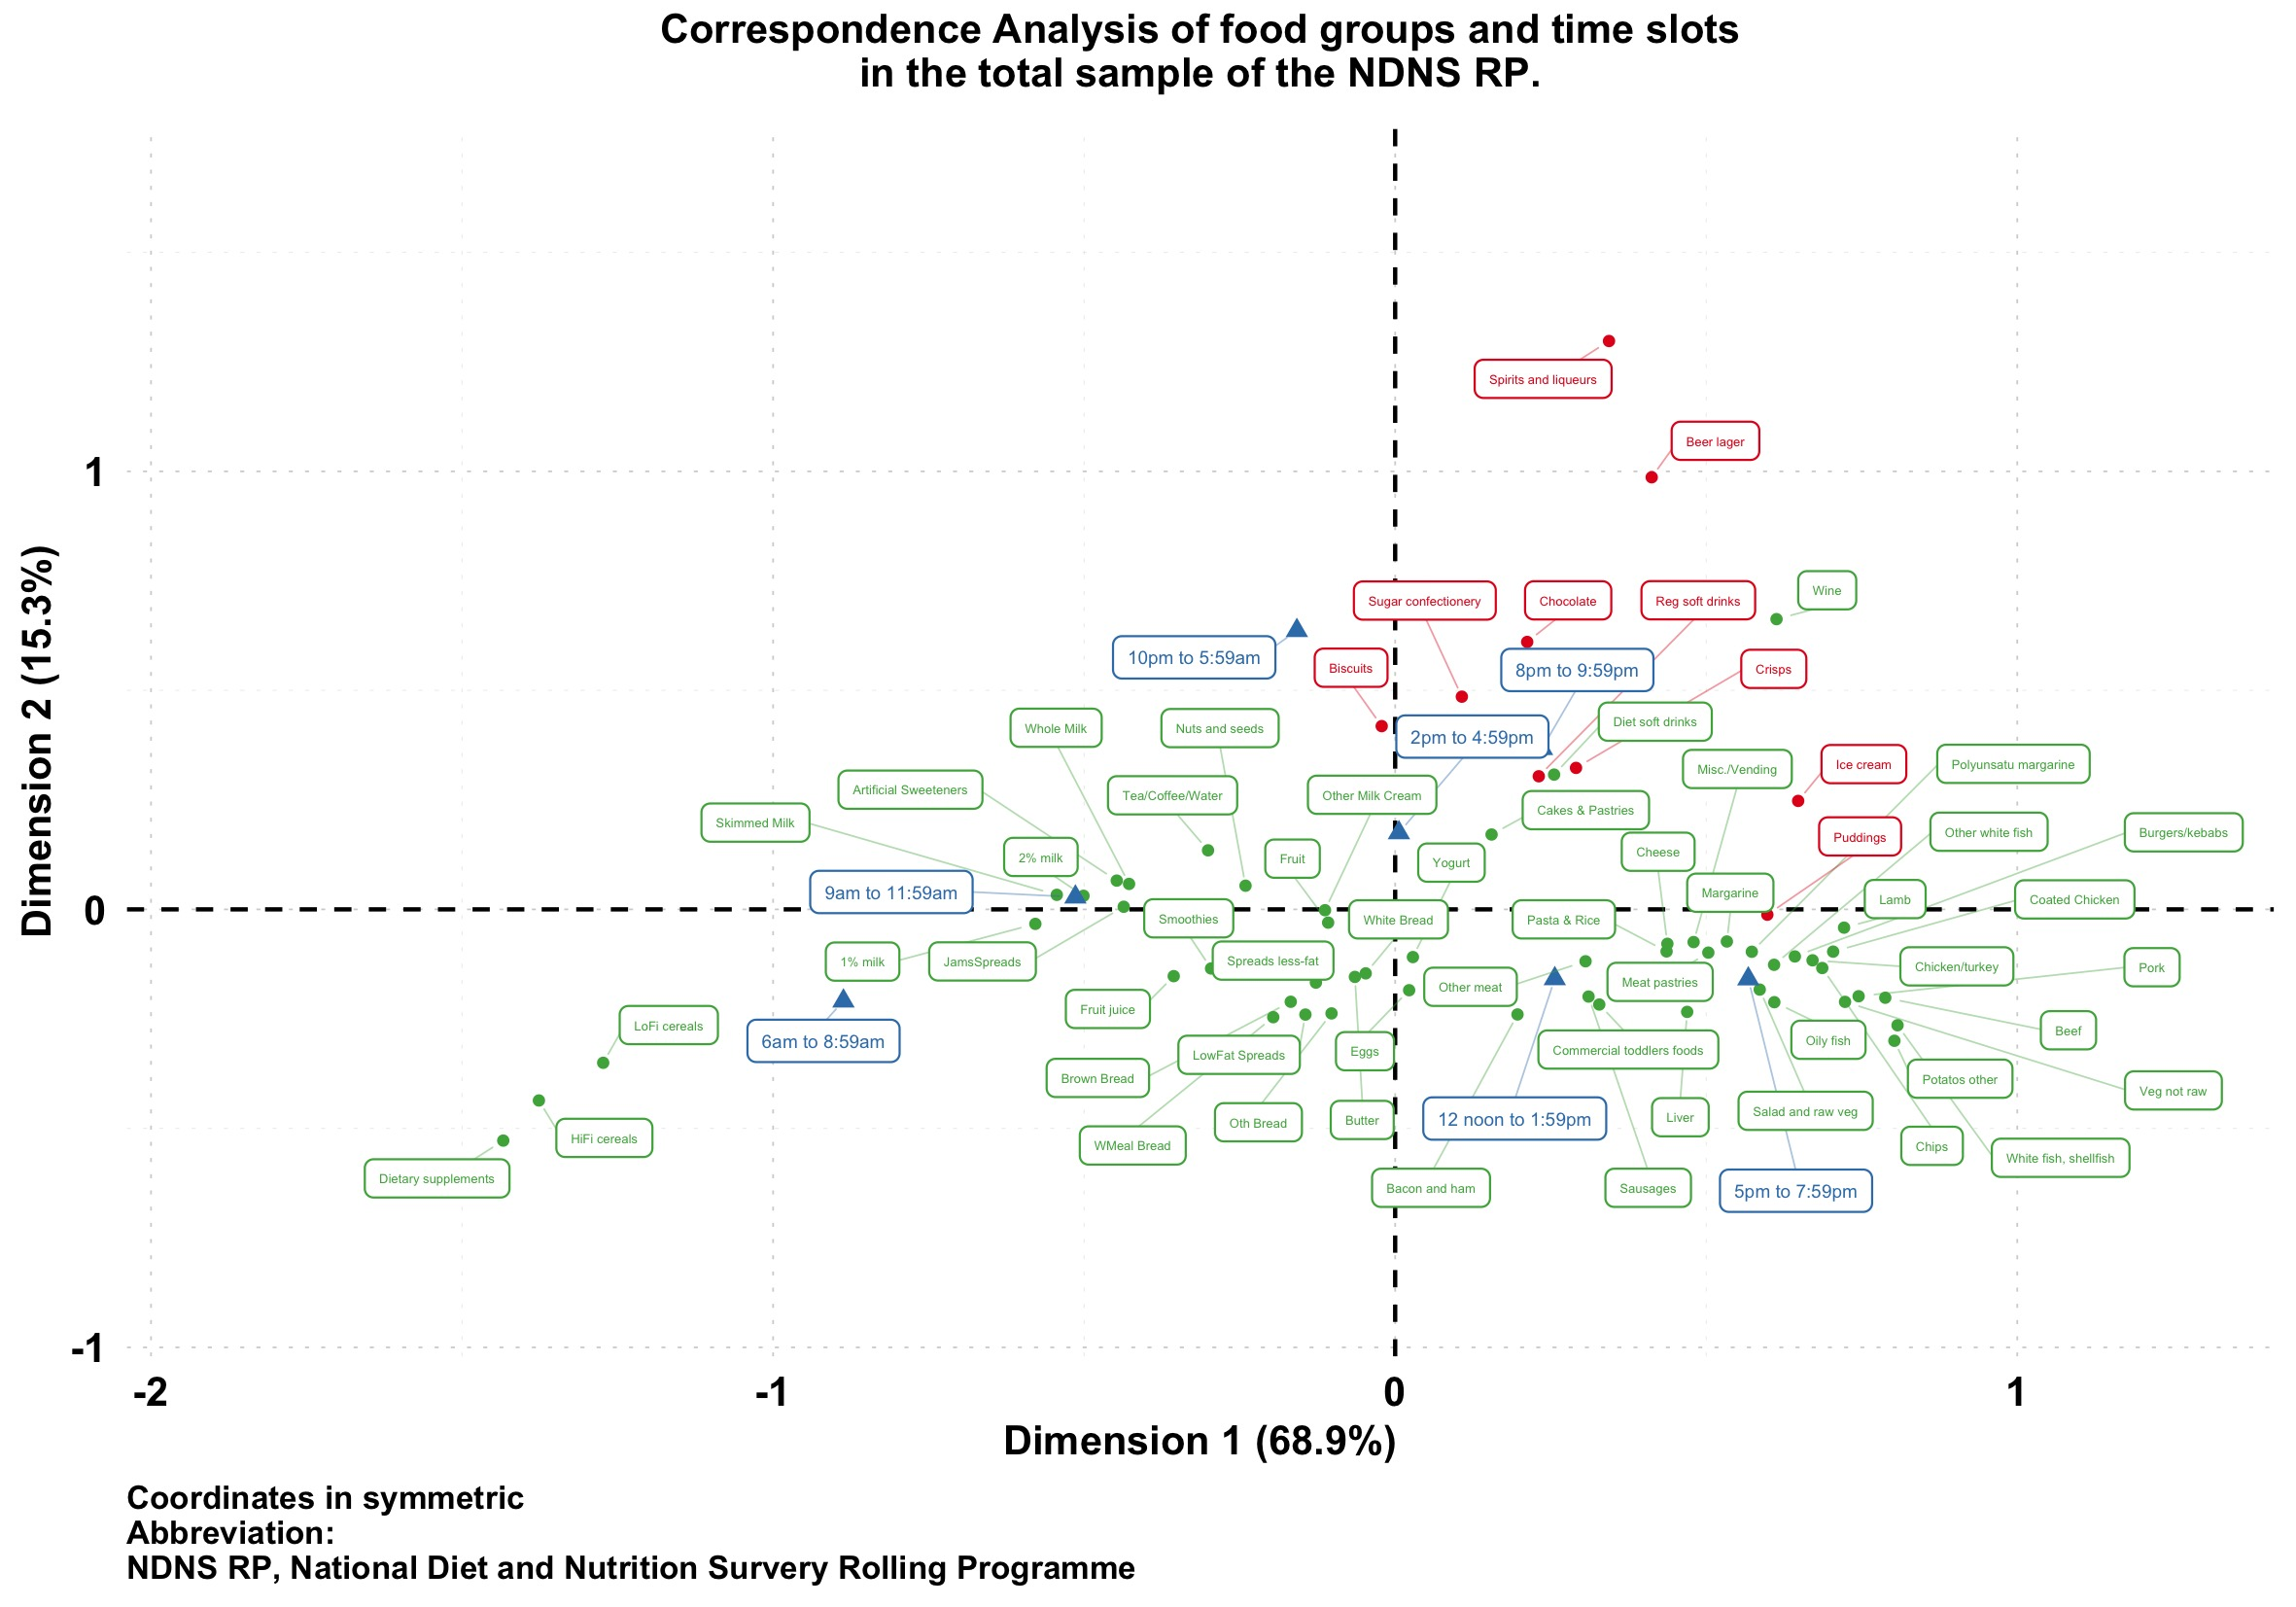
\includegraphics[width=21.5cm]{Fig1.jpg}
%DIFDELCMD < %%%
\DIFdelendFL \DIFaddbeginFL 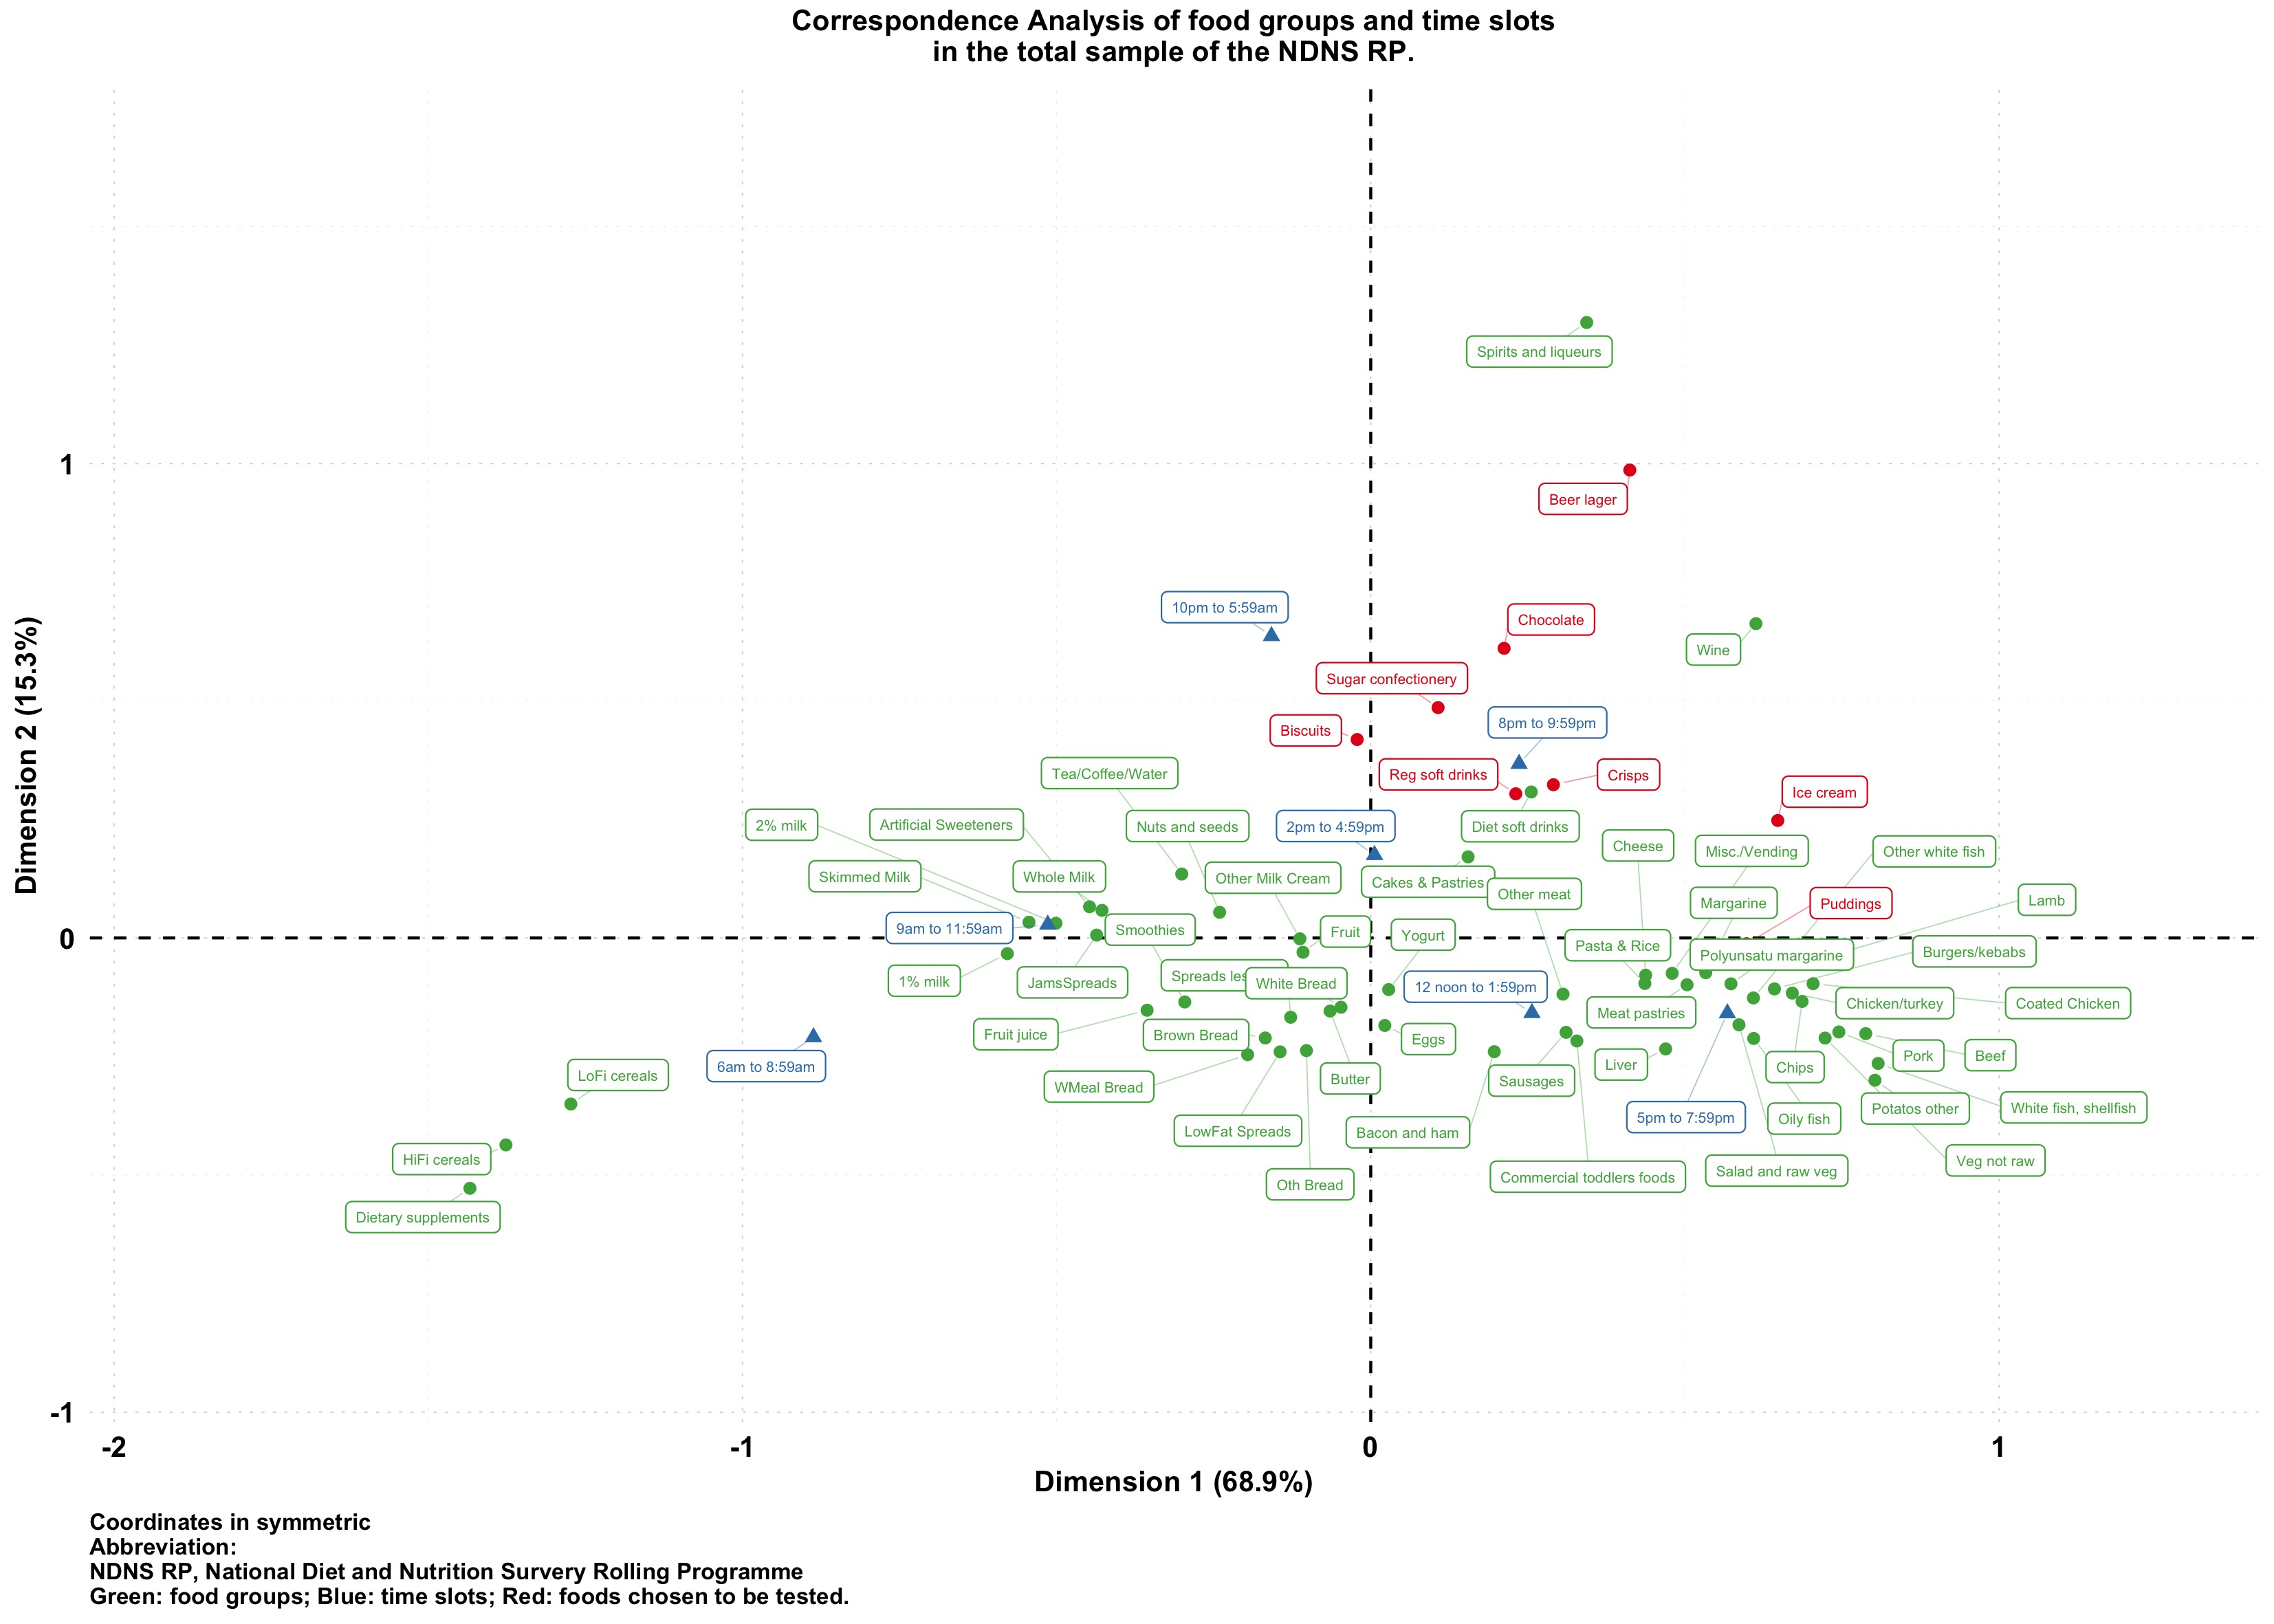
\includegraphics[width=21.5cm]{Fig1_big.jpg}
\DIFaddendFL \end{center}
\caption{Biplot of food groups and eating time slots in the total sample in the NDNS RP.}\label{fig:fig1}
\end{figure}

\begin{figure}[!ht]
\begin{center}
\DIFdelbeginFL %DIFDELCMD < 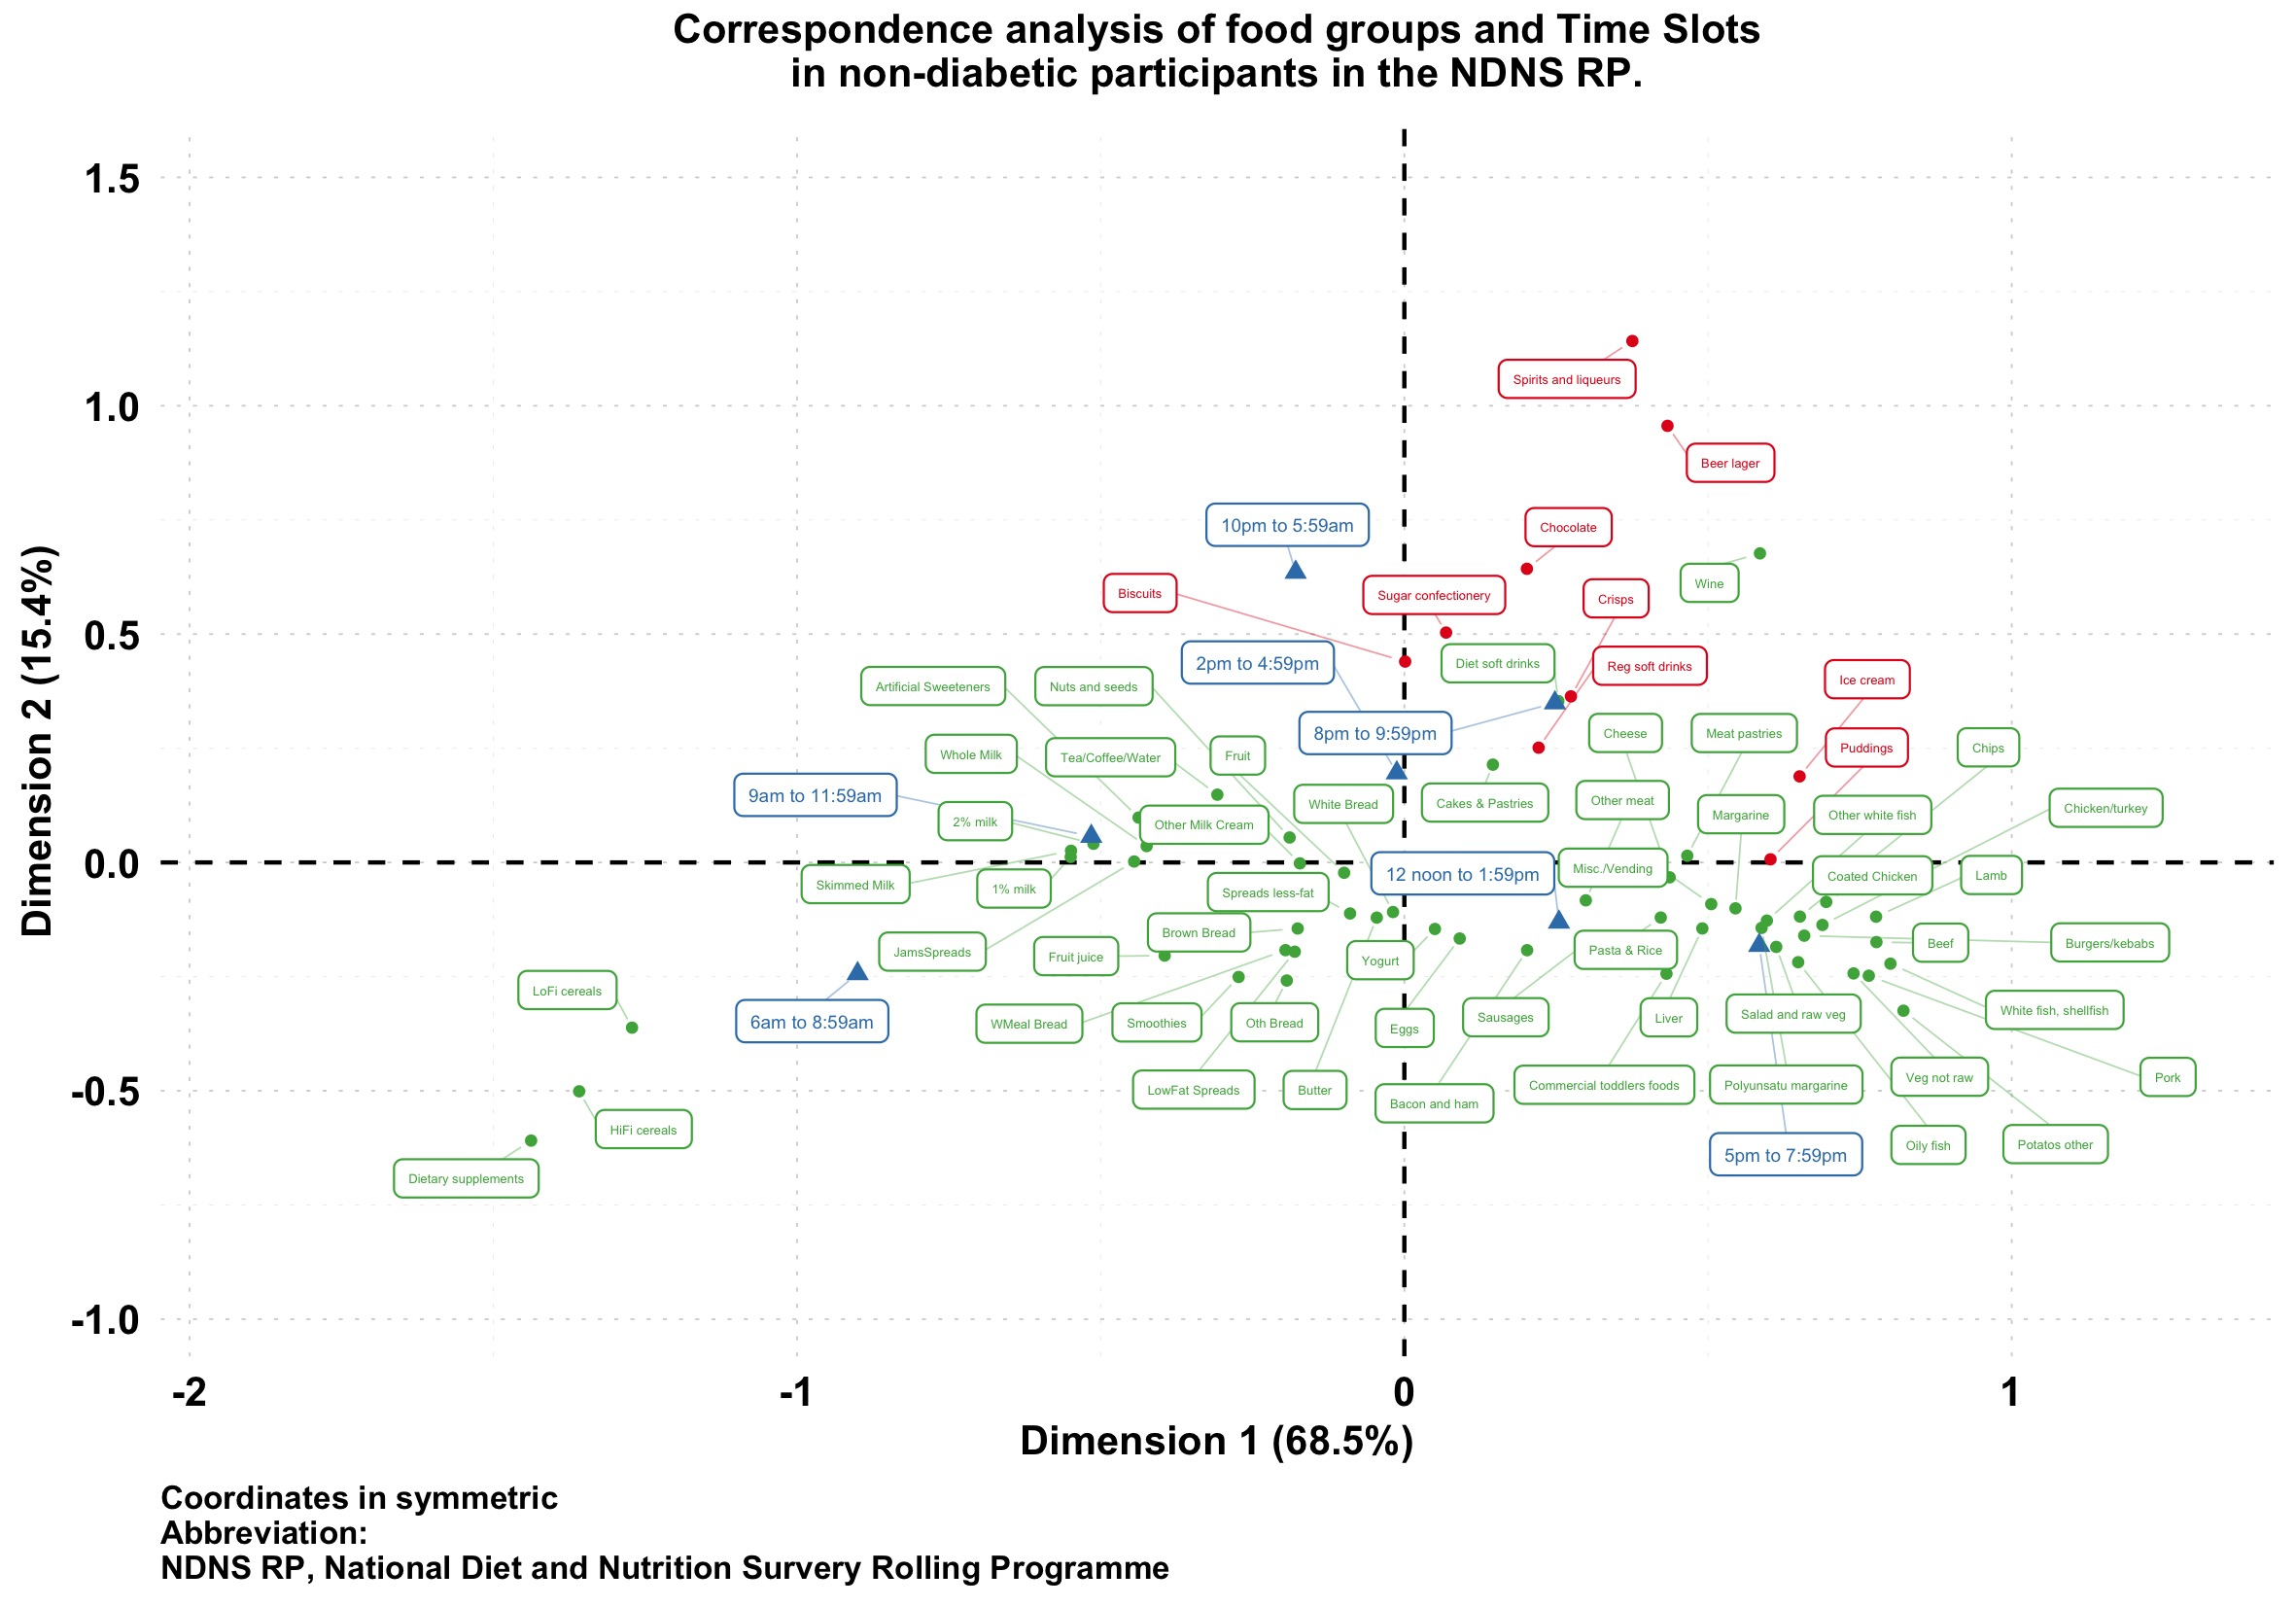
\includegraphics[width=21.5cm]{Fig2.jpg}
%DIFDELCMD < %%%
\DIFdelendFL \DIFaddbeginFL 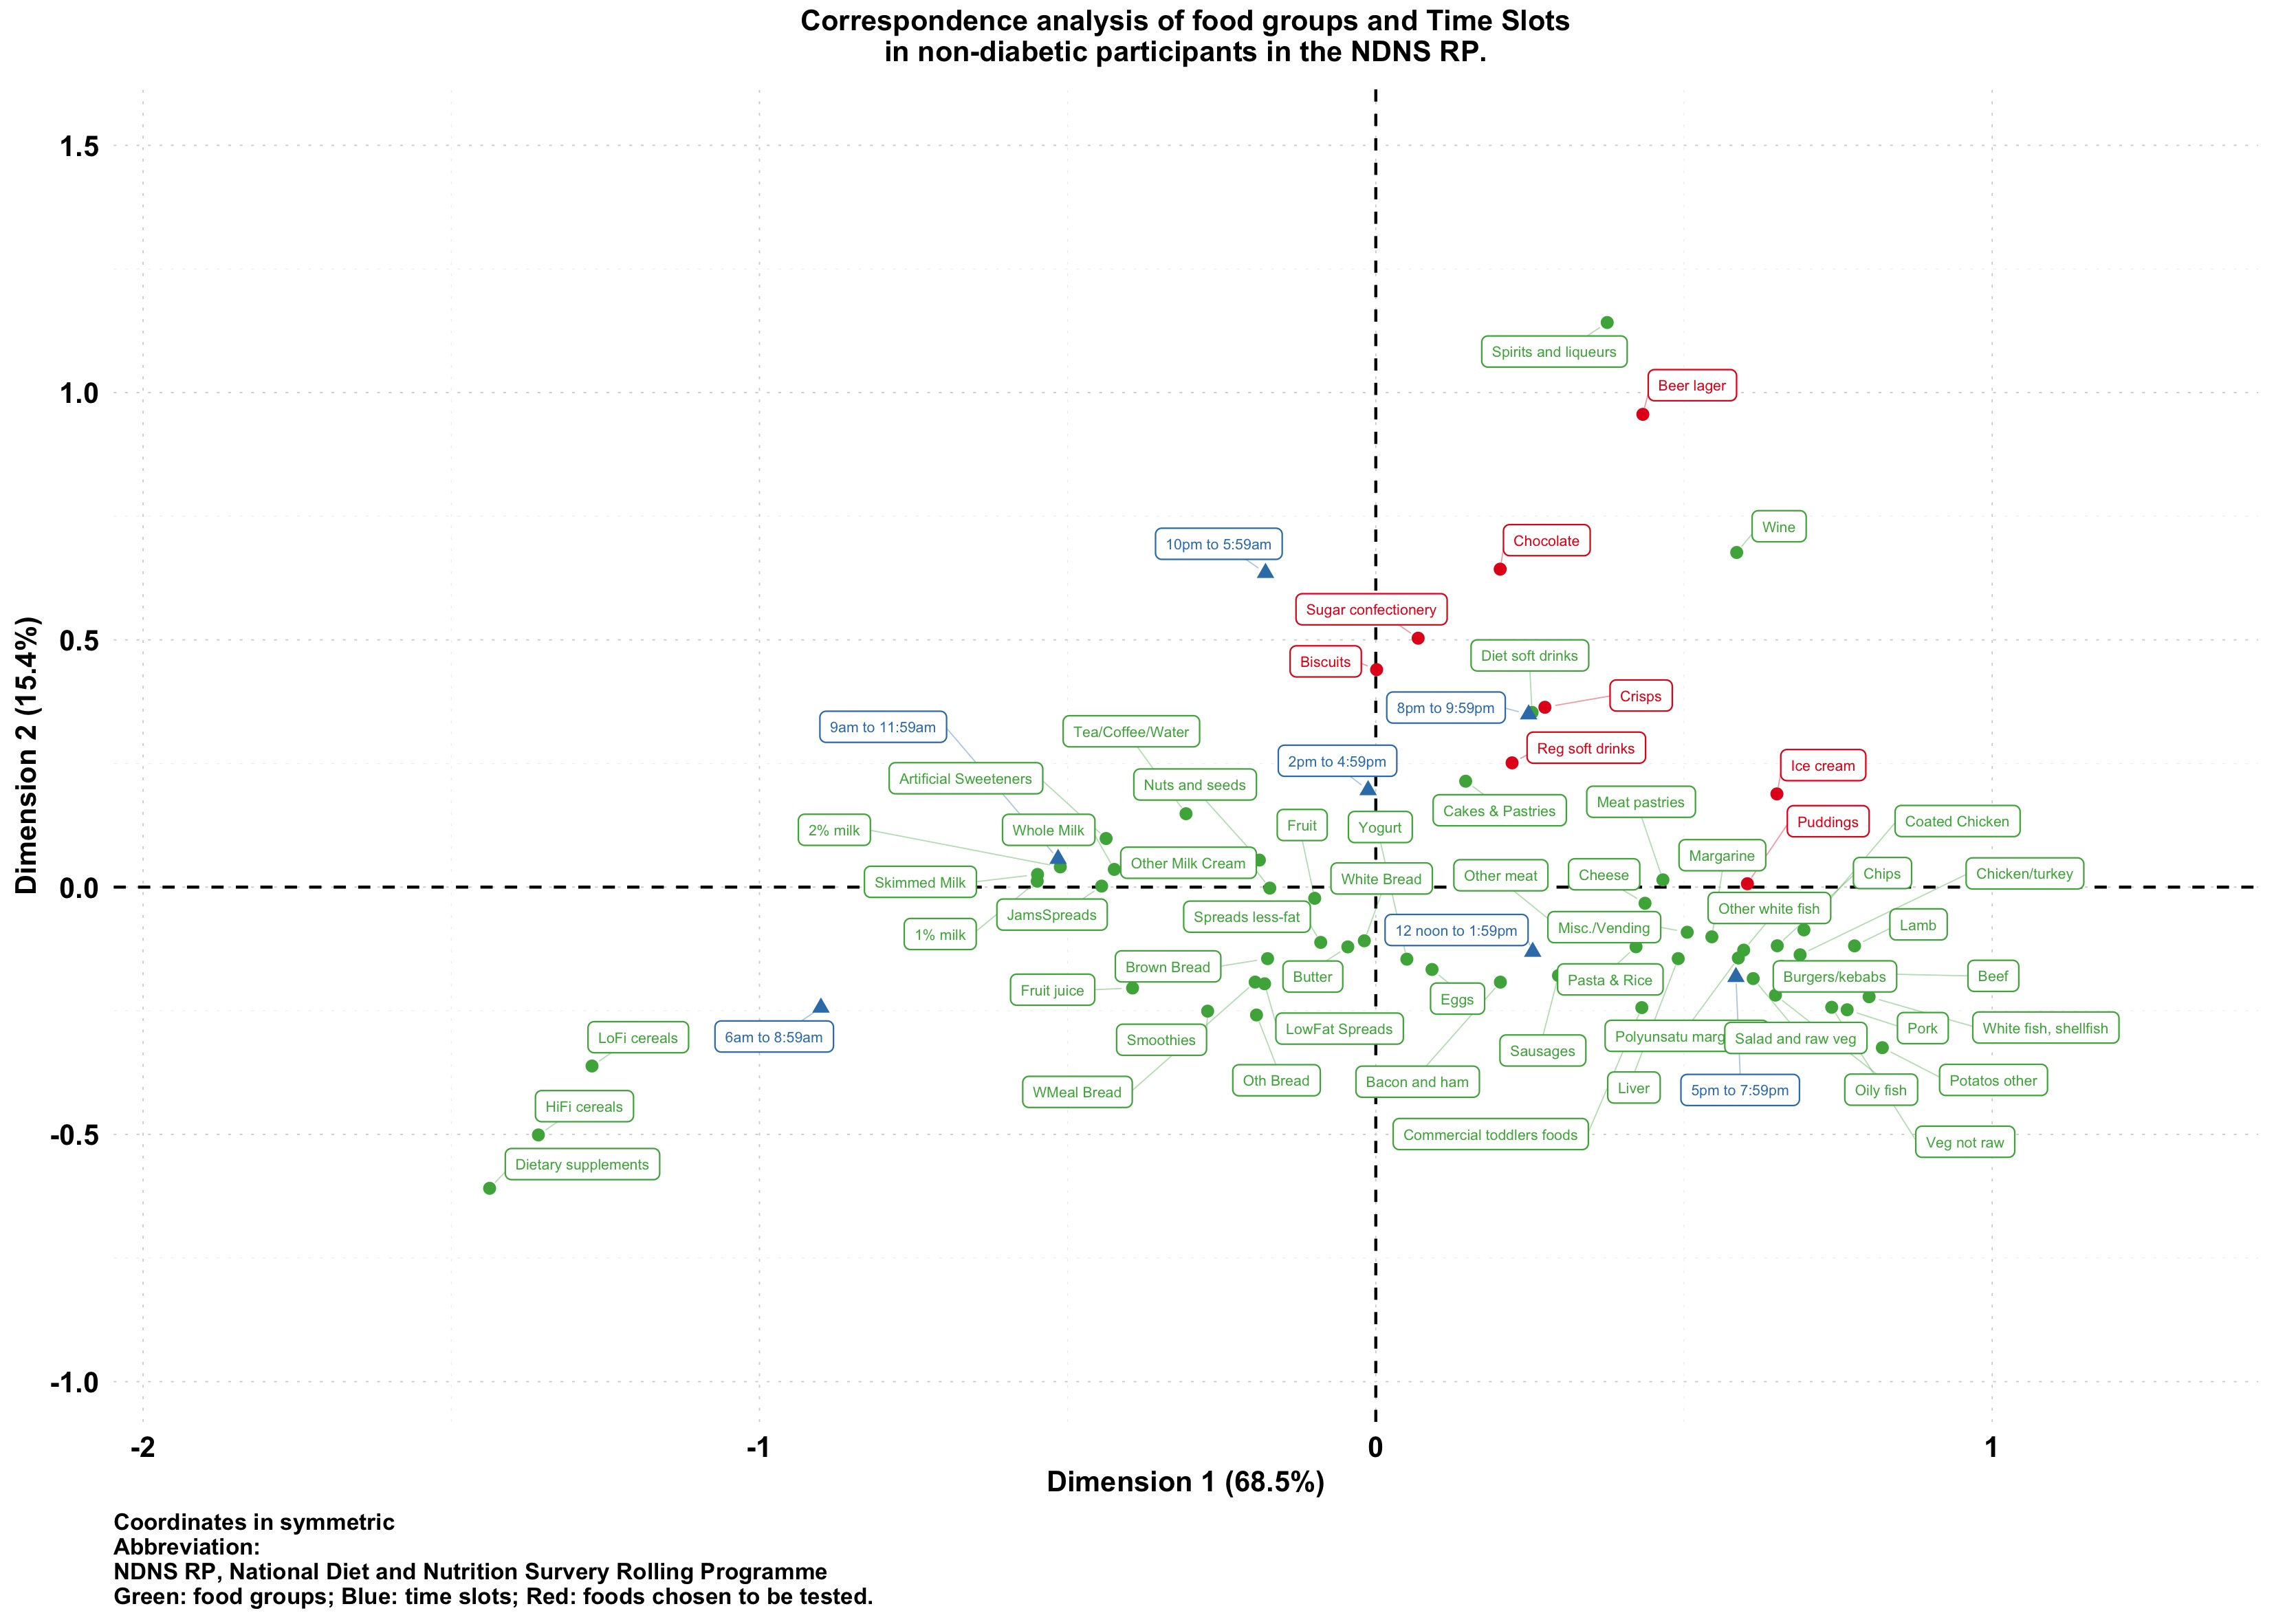
\includegraphics[width=21.5cm]{Fig2_big.jpg}
\DIFaddendFL \end{center}
\caption{Biplot of food groups and eating time slots in non-diabetic participants in the NDNS RP.}\label{fig:fig2}
\end{figure}

\begin{figure}[!ht]
\begin{center}
\DIFdelbeginFL %DIFDELCMD < 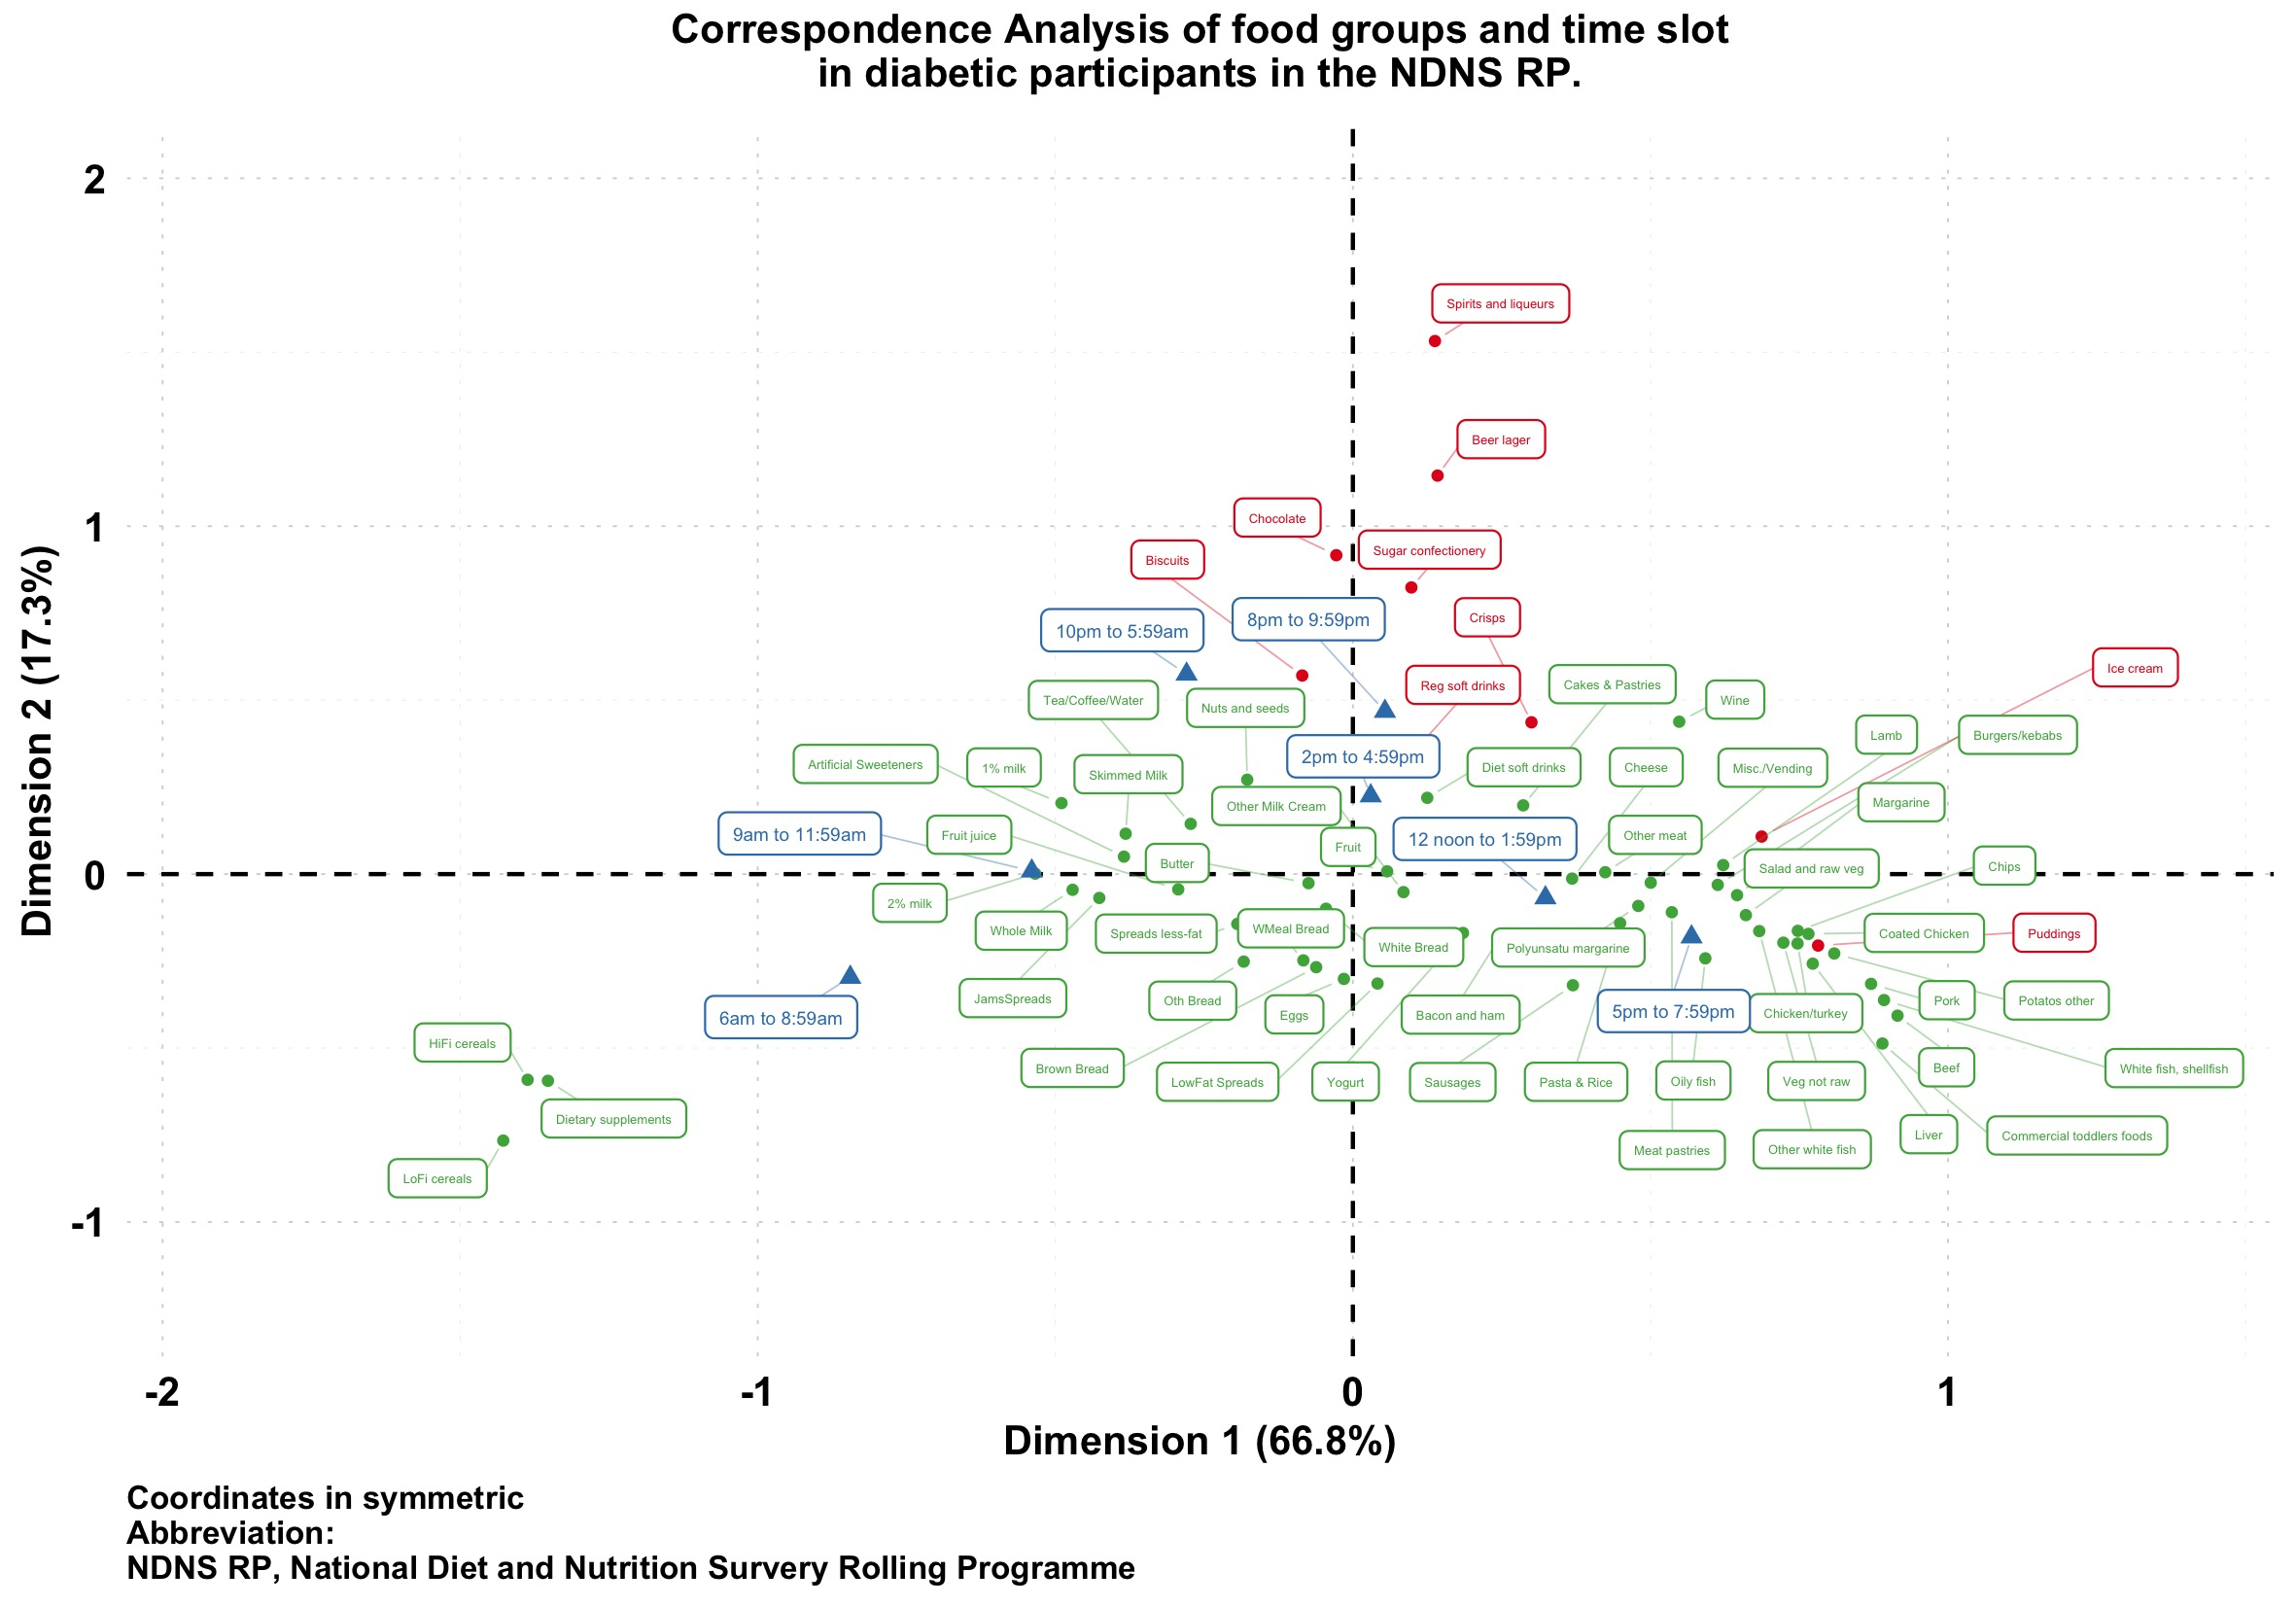
\includegraphics[width=21.5cm]{Fig3.jpg}
%DIFDELCMD < %%%
\DIFdelendFL \DIFaddbeginFL 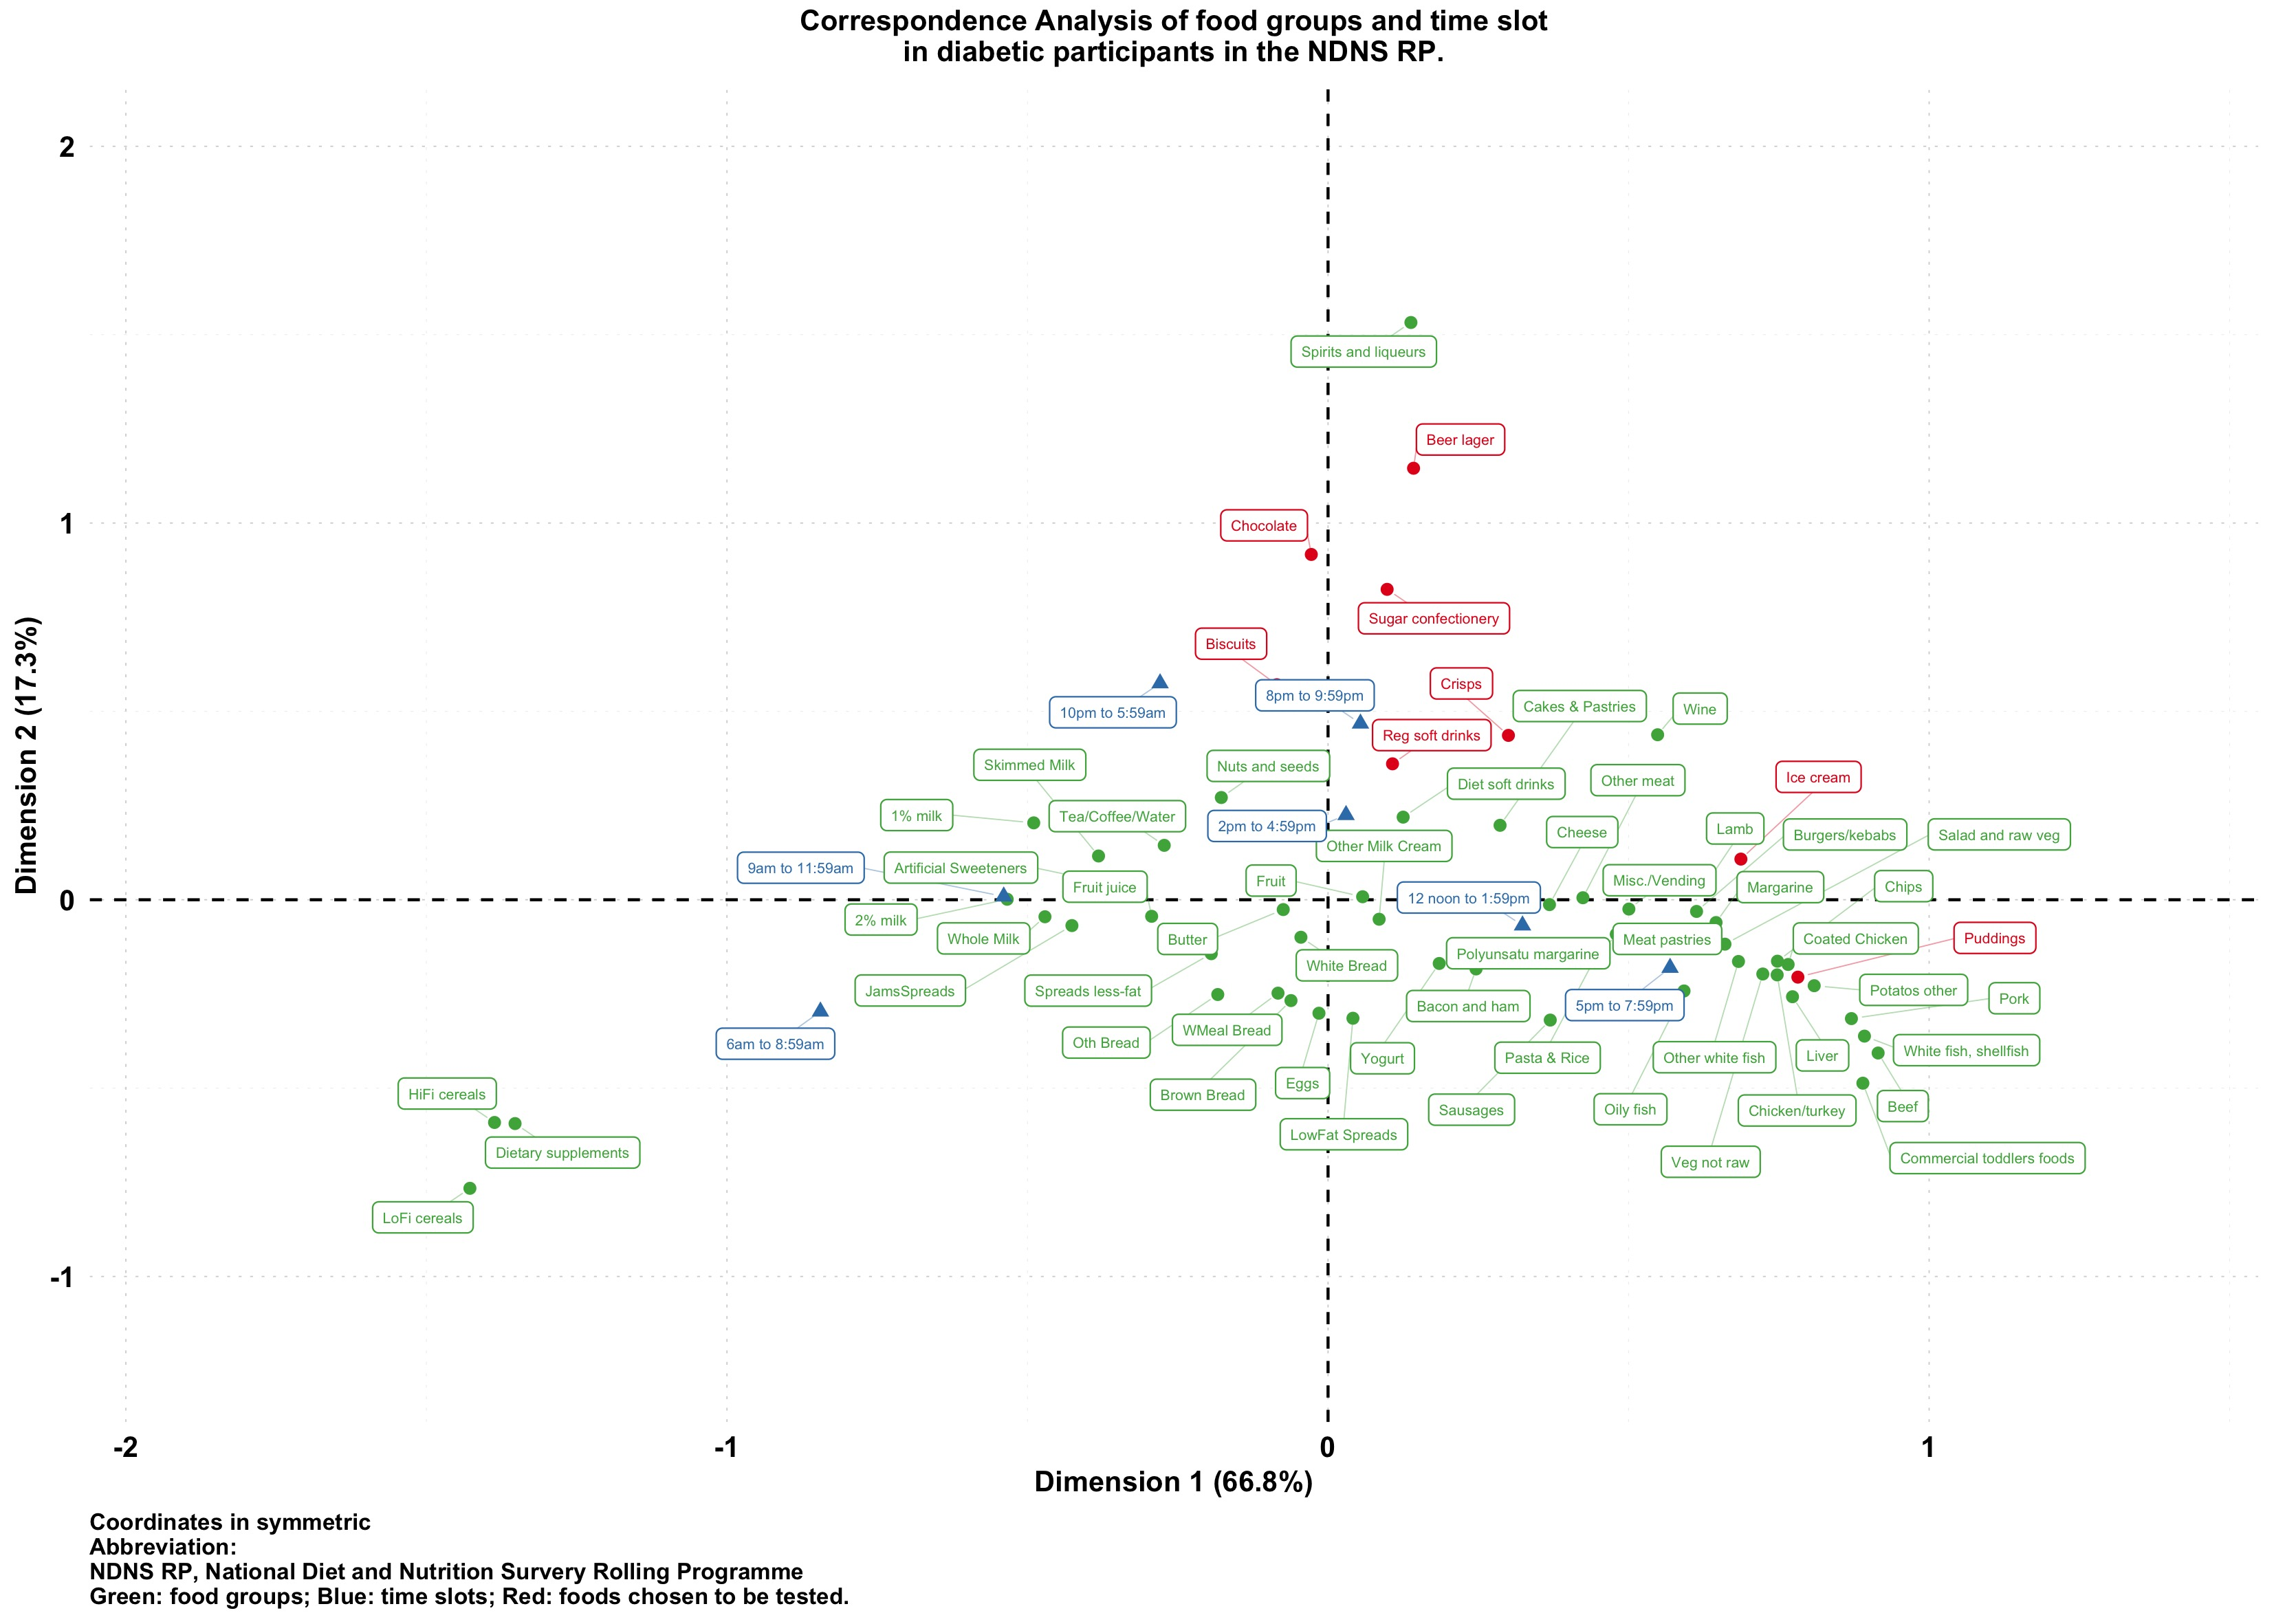
\includegraphics[width=21.5cm]{Fig3_big.jpg}
\DIFaddendFL \end{center}
\caption{Biplot of food groups and eating time slots in diabetic participants in the NDNS RP.}\label{fig:fig3}
\end{figure}

\begin{figure}[!ht]
\begin{center}
\DIFdelbeginFL %DIFDELCMD < 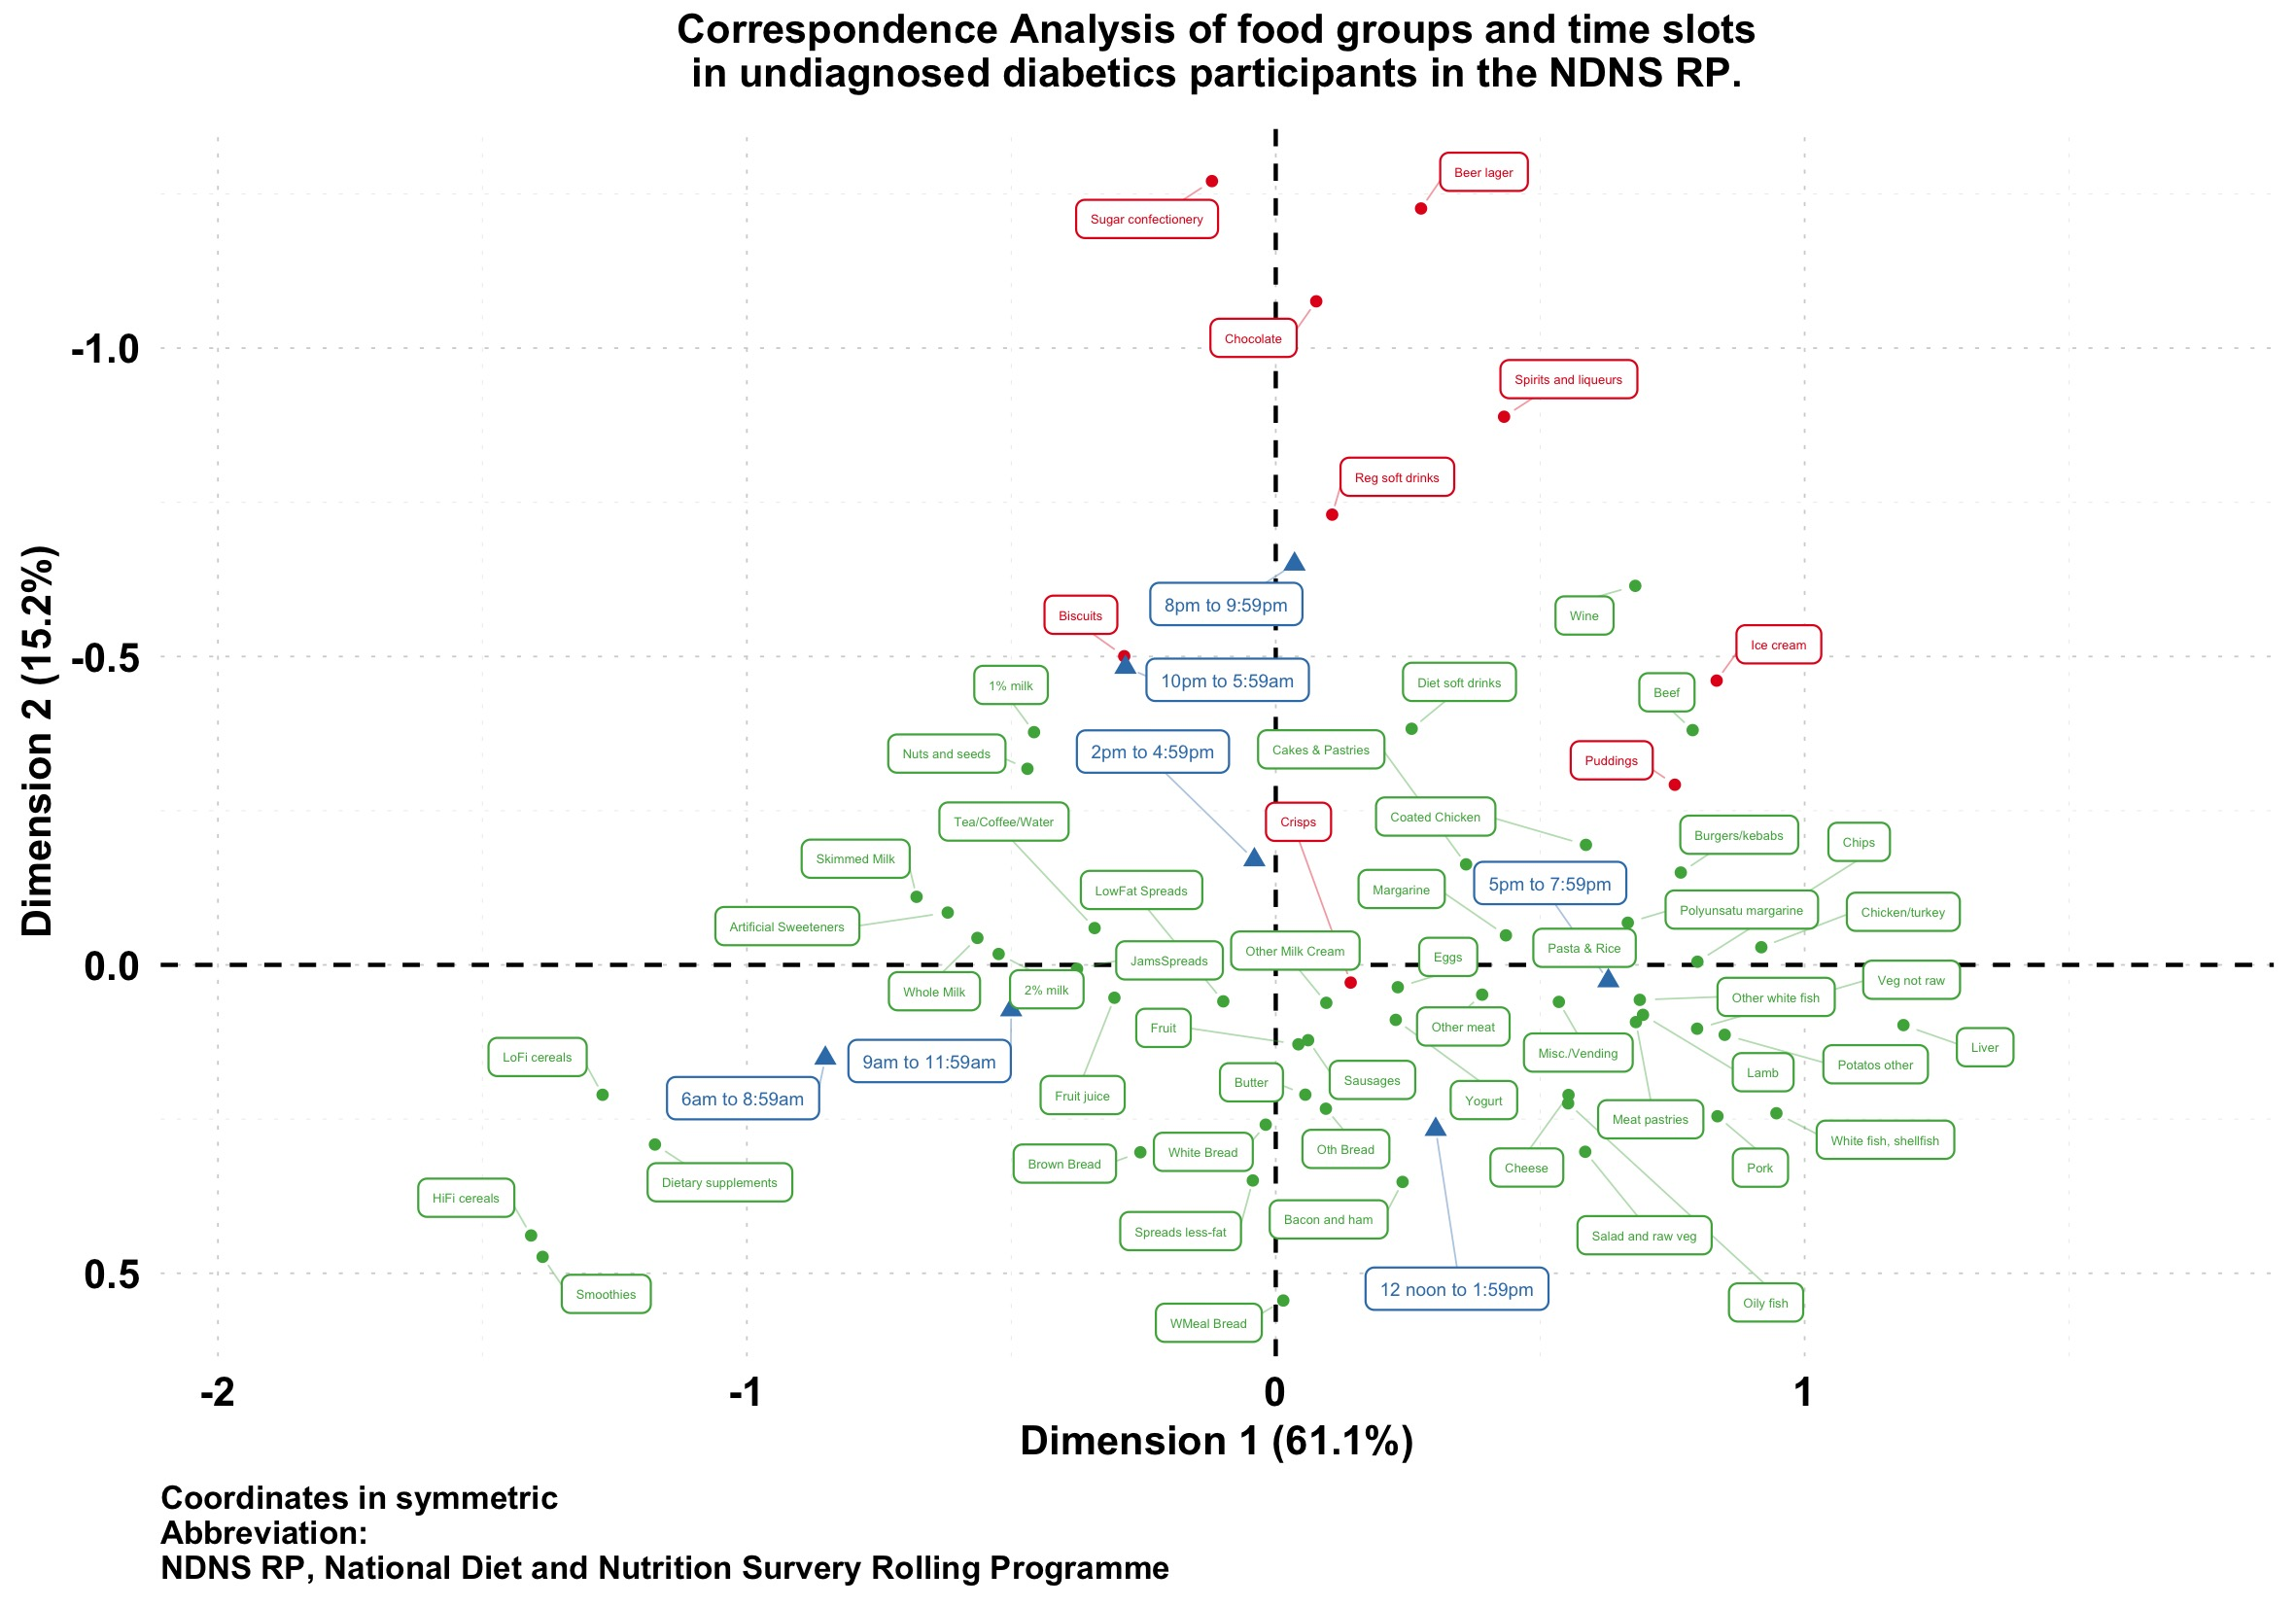
\includegraphics[width=21.5cm]{Fig4.jpg}
%DIFDELCMD < %%%
\DIFdelendFL \DIFaddbeginFL 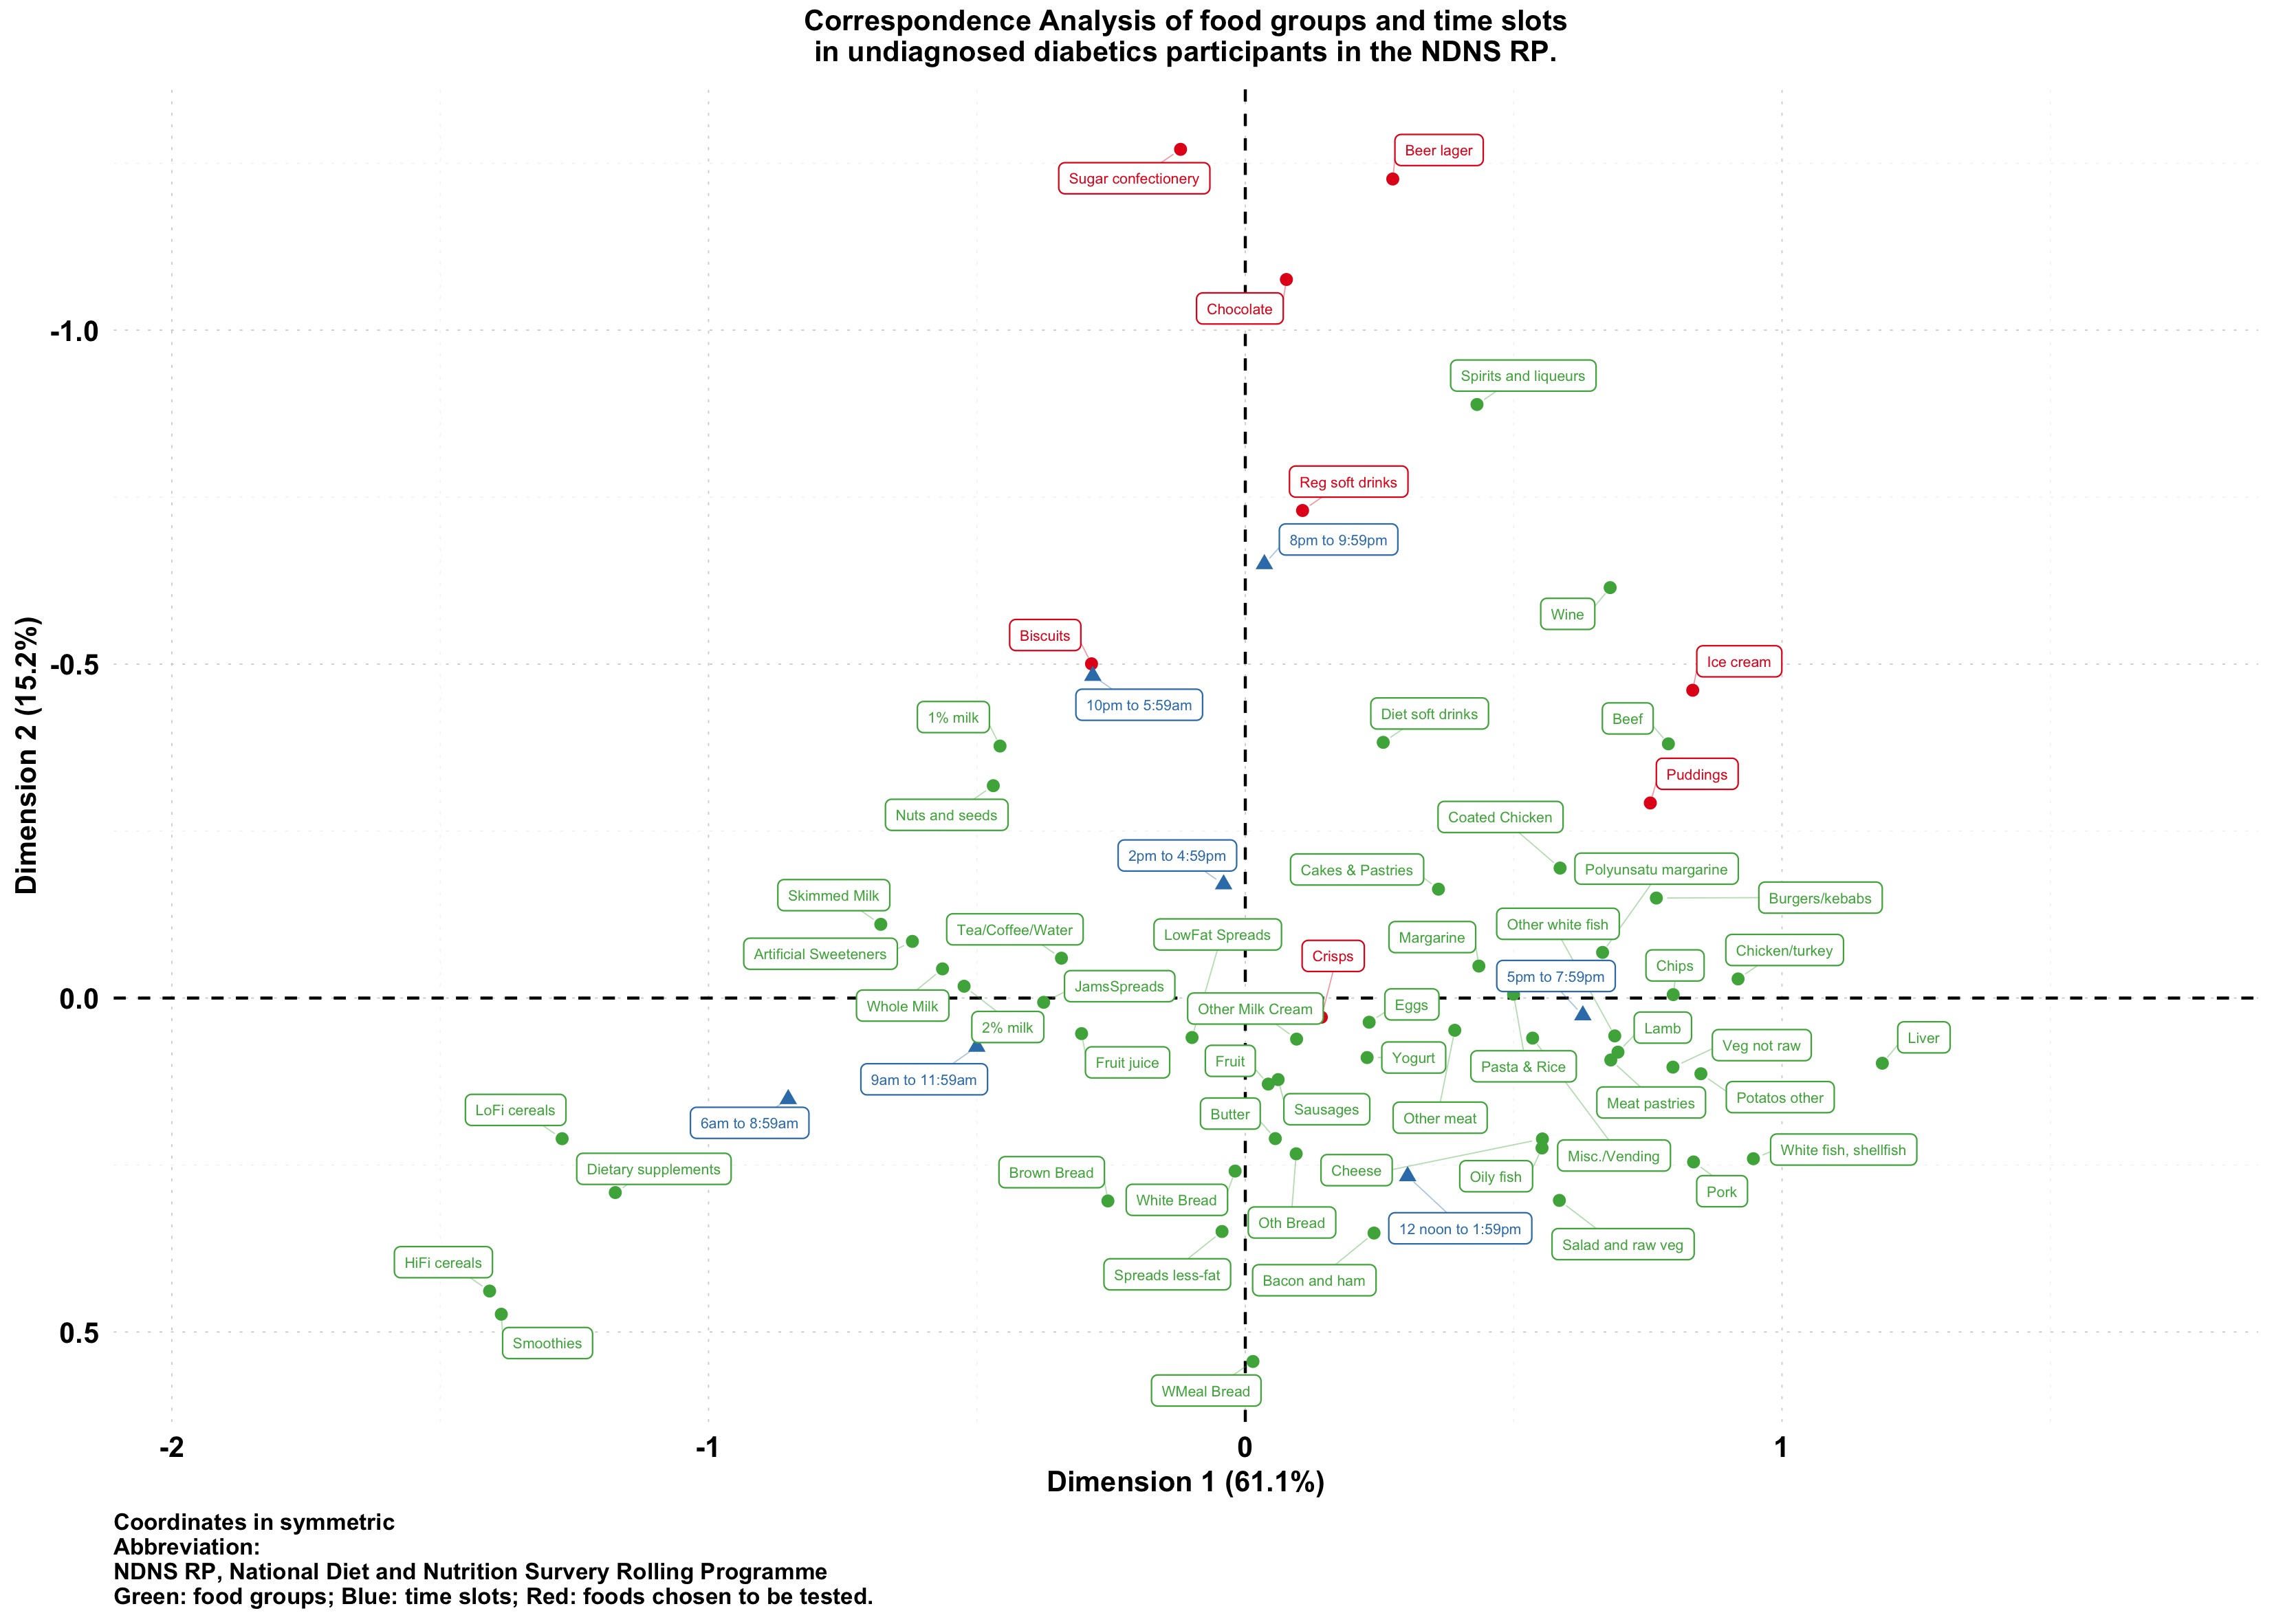
\includegraphics[width=21.5cm]{Fig4_big.jpg}
\DIFaddendFL \end{center}
\caption{Biplot of food groups and eating time slots in undiagnosed diabetic participants in the NDNS RP.}\label{fig:fig4}
\end{figure}

\begin{figure}[!ht]
\begin{center}
\DIFdelbeginFL %DIFDELCMD < 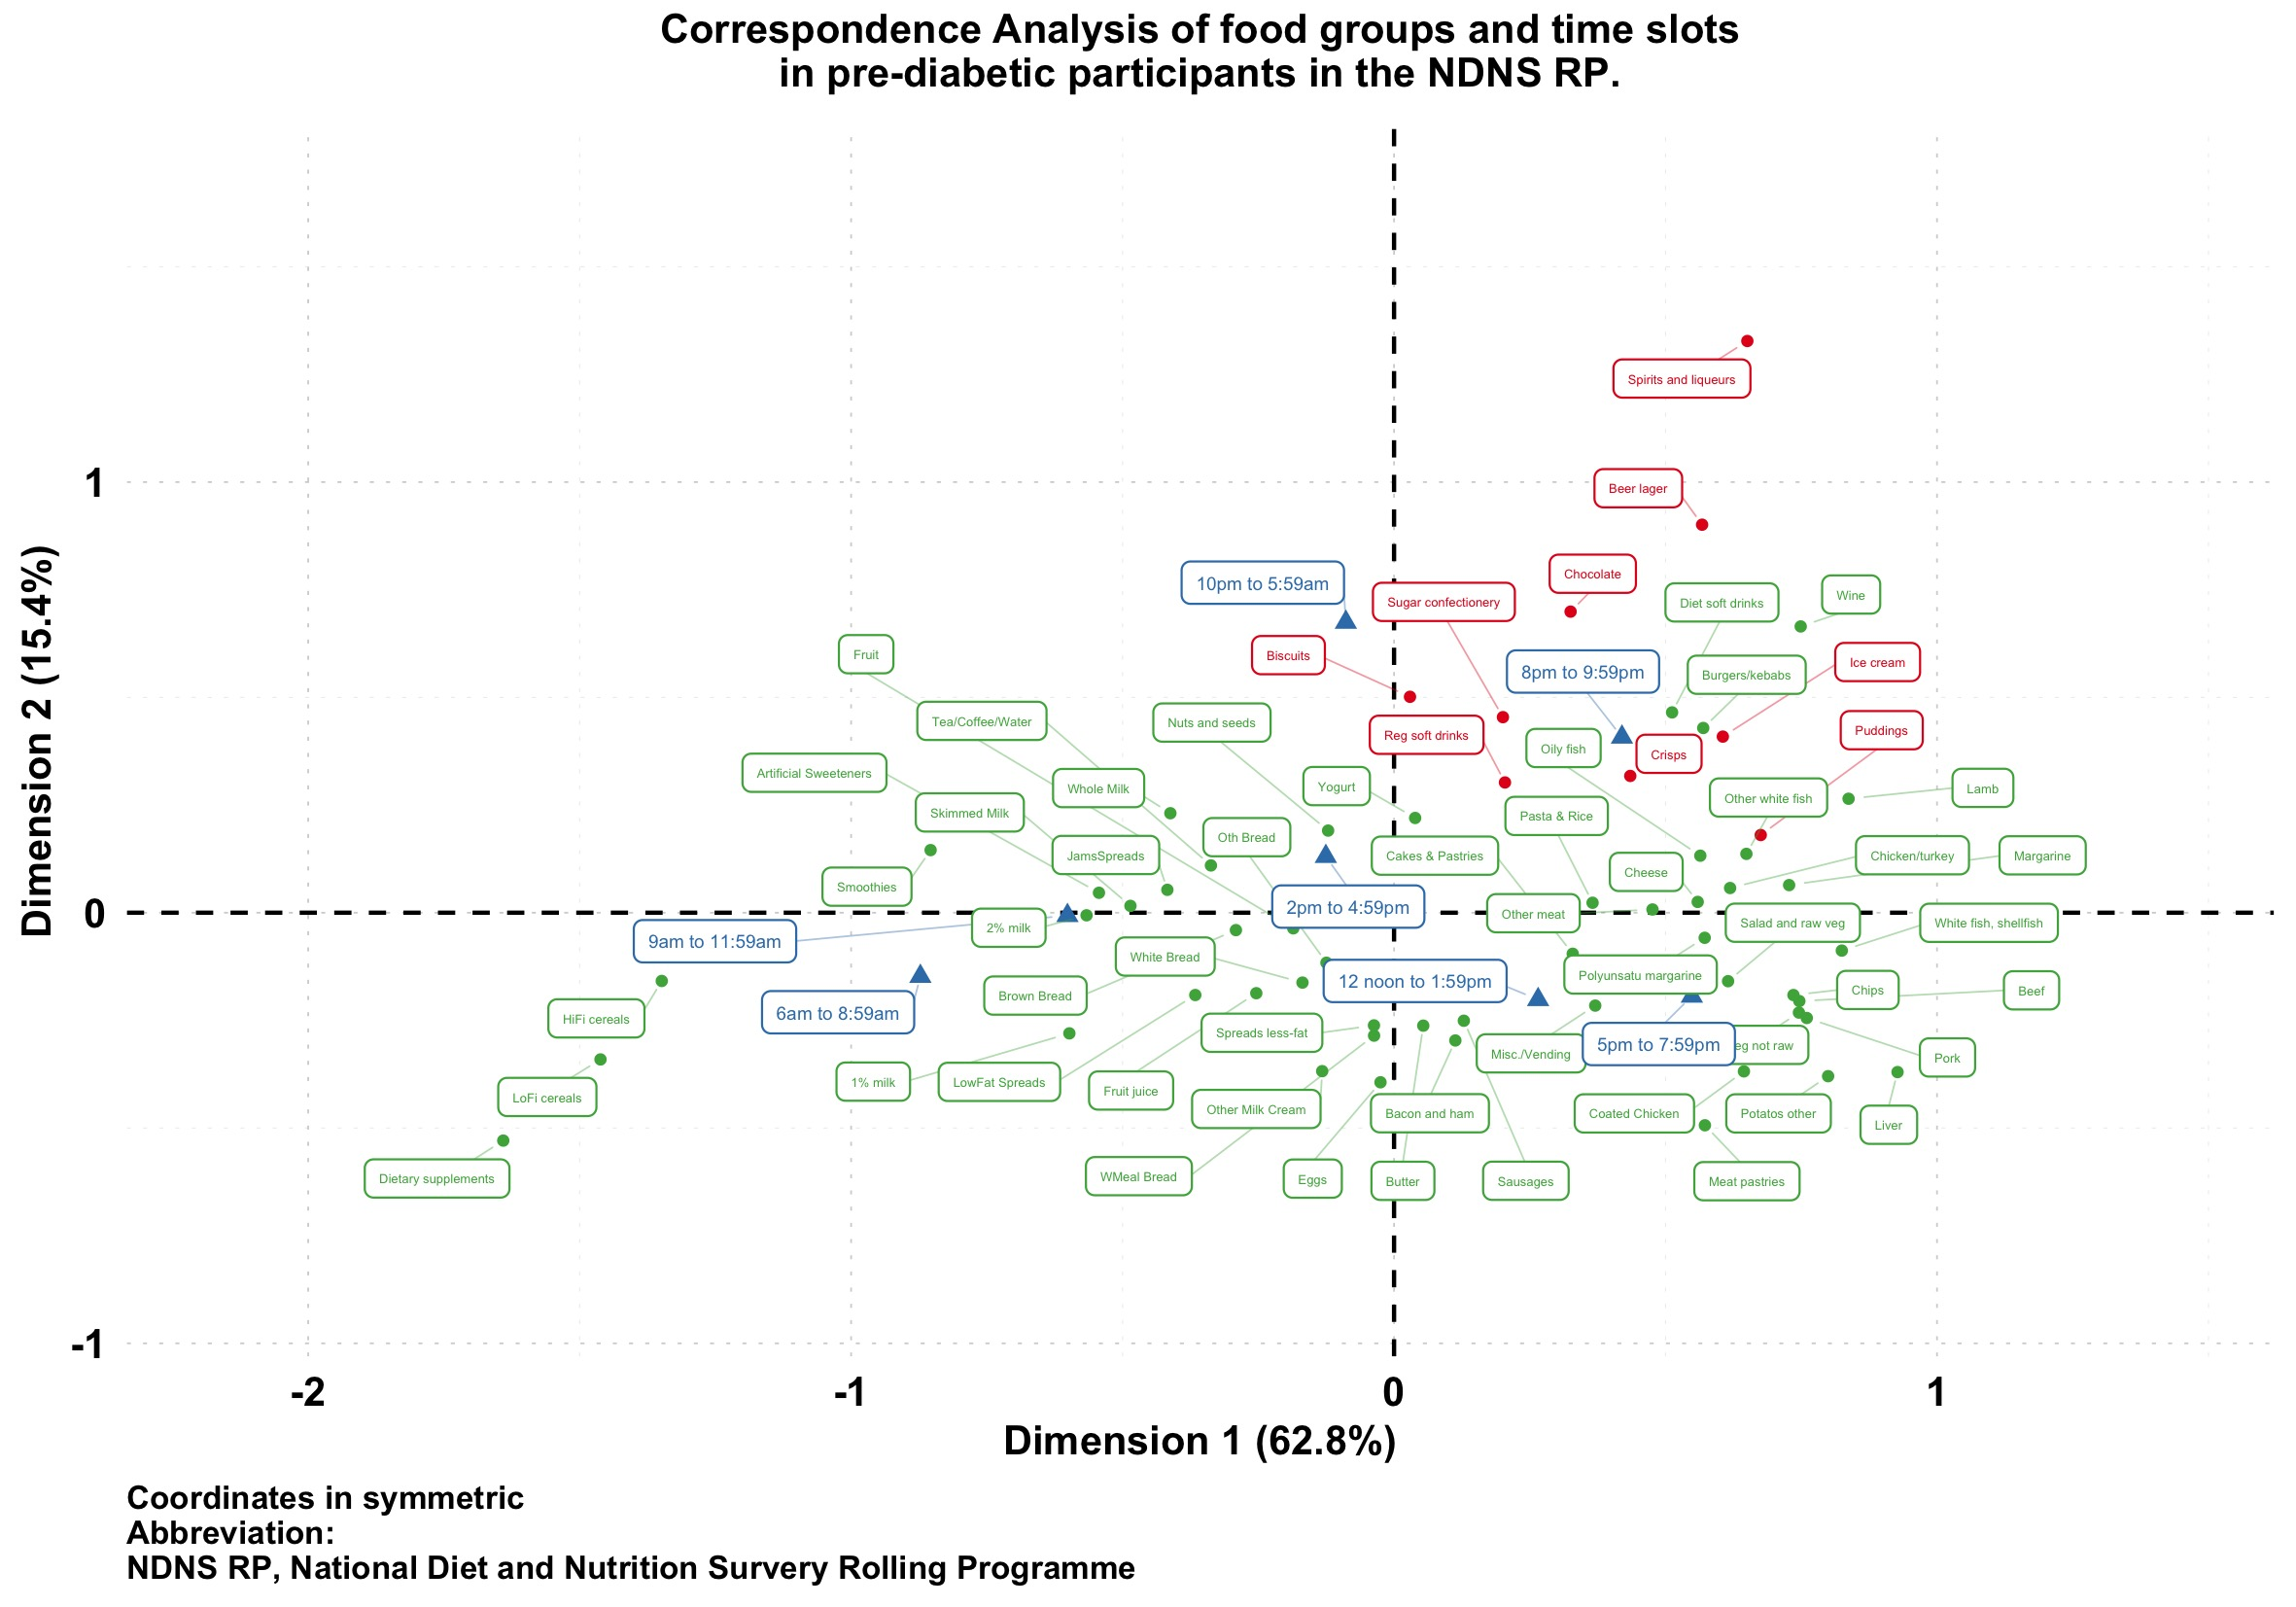
\includegraphics[width=21.5cm]{Fig5.jpg}
%DIFDELCMD < %%%
\DIFdelendFL \DIFaddbeginFL 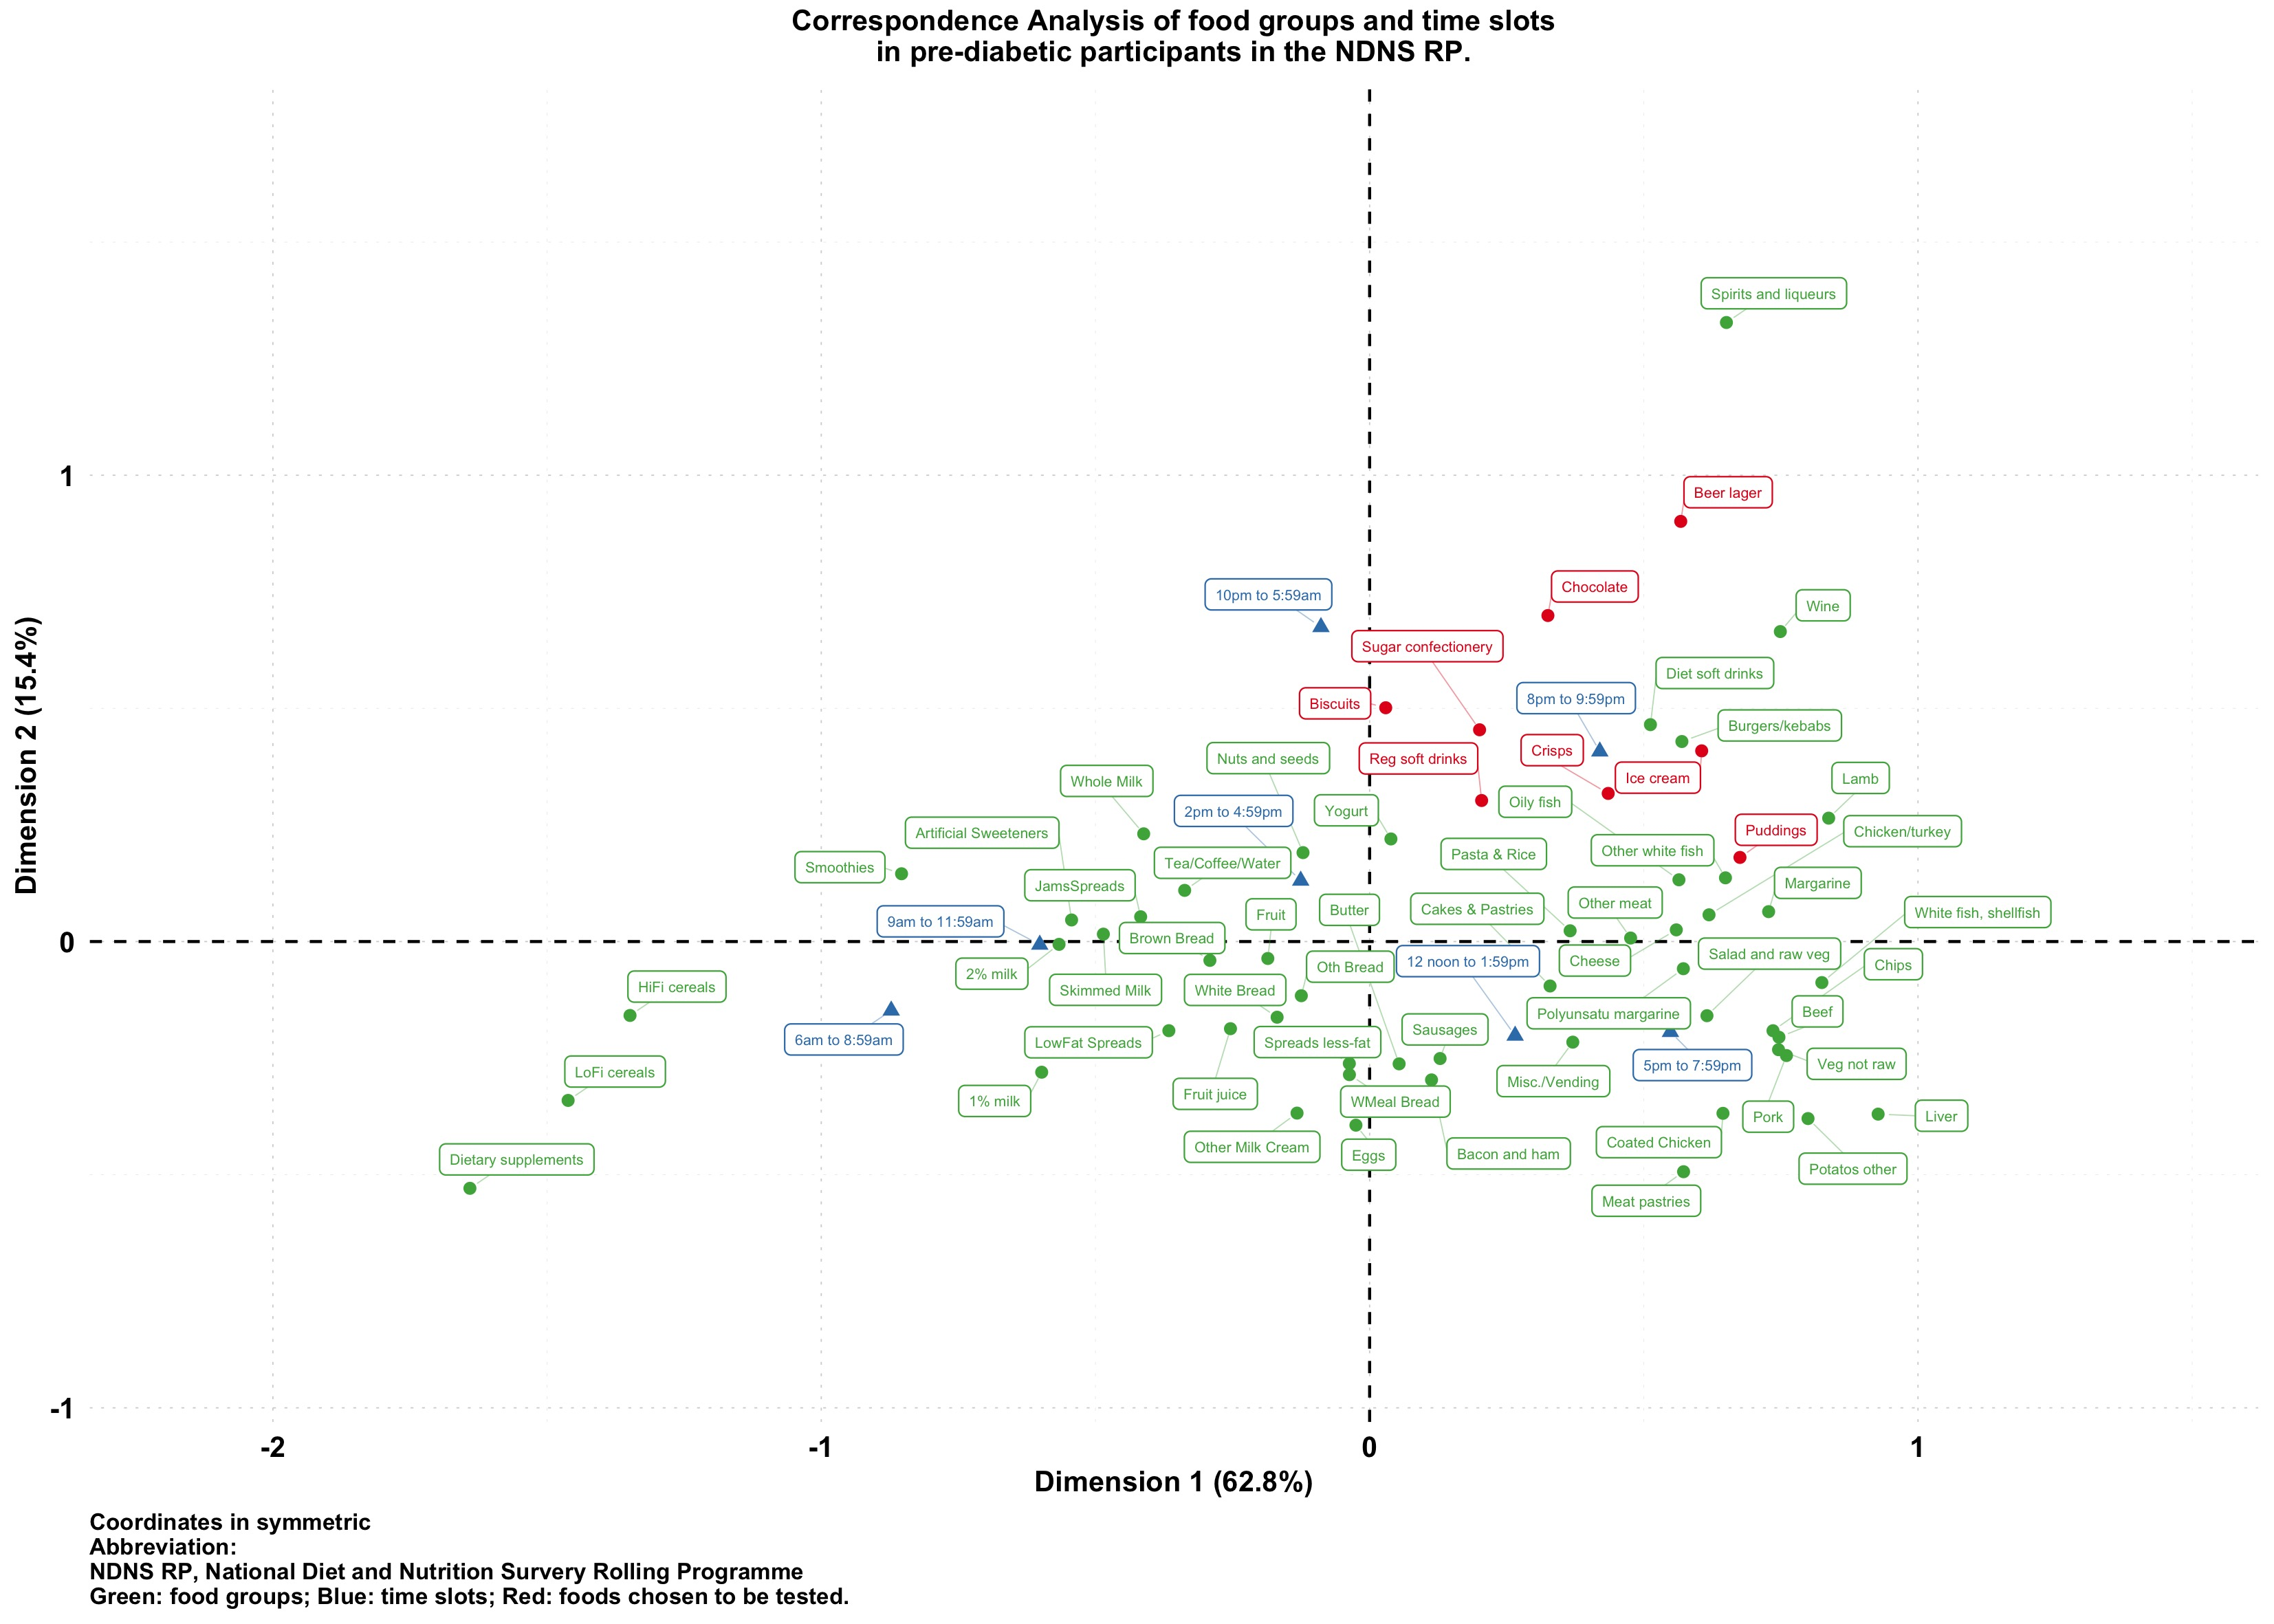
\includegraphics[width=21.5cm]{Fig5_big.jpg}
\DIFaddendFL \end{center}
\caption{Biplot of food groups and eating time slots in pre-diabetic participants in the NDNS RP.}\label{fig:fig5}
\end{figure}

\end{landscape}

\end{document}
